\documentclass[11pt]{article}
\usepackage[margin=1.8cm]{geometry}
\usepackage{graphicx}
\usepackage{booktabs}
\usepackage{longtable}
\usepackage{array}
\usepackage{xcolor}
\usepackage{hyperref}
\usepackage{amsmath,amssymb}
\hypersetup{colorlinks=true,linkcolor=blue!45!black,urlcolor=blue!45!black,pdftitle={Supplementary Material: Leakage-Aware Multi-Horizon Benchmarking of Compact Neural PV Forecasts},pdfauthor={Jiangkun Zhu, Mengling Yang, Zhicong Chen, and Lijun Wu}}
\begin{document}
\renewcommand{\thetable}{S\arabic{table}}
\renewcommand{\thefigure}{S\arabic{figure}}
\renewcommand{\theequation}{S\arabic{equation}}
\title{Supplementary Material for ``Leakage-Aware Multi-Horizon Benchmarking of Compact Neural PV Forecasts Across Technologies and Sites''}
\author{Jiangkun Zhu$^{1}$, Mengling Yang$^{1}$, Zhicong Chen$^{1,2,*}$, and Lijun Wu$^{1,2,*}$\\[0.5em]
\small $^{1}$College of Advanced Manufacturing, Fuzhou University, 1 Shuicheng Road, Quanzhou 362251, China\\
\small $^{2}$College of Physics and Information Engineering, Fuzhou University, 2 Xueyuan Road, Fuzhou 350116, China\\
\small $^{*}$Corresponding authors: zhicong.chen@fzu.edu.cn; lijun.wu@fzu.edu.cn\\
\small Jiangkun Zhu ORCID: 0009-0009-5335-2345}
\date{}
\maketitle

\section{Evidence scope}
This supplement reports the frozen evidence supporting the main manuscript. The benchmark comprises three co-located Alice Springs arrays (36 runs, 17 channels) and two separately fitted external facilities, Yulara and NIST Ground (24 runs, seven channels). Each experiment uses four compact neural implementations, seeds 42, 43, and 44, and direct 144-step forecasts at five-minute resolution. Primary H12, H48, H96, and H144 metrics use horizon-specific valid origins. Daily Persistence comparisons instead use an elementwise intersection mask that is valid for the daily lag, labels, Last-value Persistence, and every neural forecast.

\section{Input and preprocessing configuration}
For Alice Springs, each history has 72 time steps and 17 channels: Performance Ratio; ambient temperature; relative humidity; global and diffuse horizontal radiation; global and diffuse tilted radiation; Active Power; eight corresponding missingness indicators; and one Isolation Forest indicator. The imputer, feature scaler, target scaler, and Isolation Forest are fitted on Train only. No forecast-origin successor value enters the input. Windows remain within chronological splits and within a regular five-minute coordinate.

\begin{table}[h]
\caption{Fixed optimization configuration for all compact neural implementations.}
\par\small\textit{Alt text: The shared optimization configuration fixes the optimizer, learning rate, batch size, epoch budget, early-stopping rule, gradient clipping, H144 validation objective, and three random seeds for all four compact implementations.}\par
\centering
\begin{tabular}{ll}
\toprule Setting & Value\\
\midrule
Optimizer & AdamW\\
Learning rate & $10^{-3}$\\
Weight decay & $10^{-5}$\\
Batch size & 256\\
Maximum epochs & 25\\
Early-stopping patience & 5\\
Minimum improvement & $10^{-8}$\\
Gradient clipping & 1.0\\
Checkpoint objective & Validation global masked MSE on H144\\
Random seeds & 42, 43, 44\\
\bottomrule
\end{tabular}
\end{table}

\section{Architecture identity and full layer configuration}
The Discrete recurrent decoder combines three temporal-convolution branches (dilations 1, 2, and 4; 24 channels each), a 64-dimensional one-layer Transformer, a learned feature gate, bidirectional GRU attention, and an autoregressive GRUCell trajectory decoder. The Inverted-variate Transformer treats the 17 Alice or seven external channels as tokens, projects each 72-point history to 64 dimensions, applies one four-head Transformer layer, then flattens the encoded tokens into a 144-output linear map. The Joint-patch Transformer forms overlapping joint multivariate patches of length 12 and stride 6, uses one 64-dimensional four-head Transformer layer, and maps the encoded patches to 144 outputs. The Depthwise TCN uses an input projection followed by four depthwise-separable temporal blocks with 64 channels and kernel size 5, then a flattened linear H144 head.

These are project implementations for a controlled mechanism comparison. The inverted model omits the full official iTransformer embedding, normalization, and decoder design; the joint-patch model does not use the channel-independent PatchTST pipeline; and the depthwise model omits the full ModernTCN large-kernel and multi-scale block system. Accordingly, the reported rankings do not rank the official architectures.

\section{Metrics and masks}
For a fixed valid-point set $\mathcal{I}$ with $n=|\mathcal{I}|$,
\begin{align}
\mathrm{RMSE}&=\sqrt{n^{-1}\sum_{i\in\mathcal{I}}(\hat y_i-y_i)^2},\\
\mathrm{MAE}&=n^{-1}\sum_{i\in\mathcal{I}}|\hat y_i-y_i|,\\
R^2&=1-\frac{\sum_{i\in\mathcal{I}}(\hat y_i-y_i)^2}{\sum_{i\in\mathcal{I}}(y_i-\bar y)^2},\\
\mathrm{range\mbox{-}nRMSE}&=\frac{\mathrm{RMSE}}{y_{\max,\mathrm{Train}}-y_{\min,\mathrm{Train}}},\\
\mathrm{RMSE\ skill}&=1-\frac{\mathrm{RMSE}_{\mathrm{model}}}{\mathrm{RMSE}_{\mathrm{reference}}}.
\end{align}
The daylight mask is true target Active Power greater than 1\% of the corresponding array's Train maximum. It is an evaluation-only mask. Daily Persistence takes each target timestamp's power 24 hours earlier without interpolation. If that point is unavailable, it is removed from every method in that Daily-matched comparison.

\section{Alice Springs quantitative evidence}
The following tables are generated directly from the frozen \texttt{corrected\_metrics.csv}; they are not transcribed into this source file. They provide per-seed primary metrics, primary support, complete-H144-origin sensitivity, and matched Daily Persistence results.

% AUTO-GENERATED by build_figures.py from corrected_metrics.csv. DO NOT EDIT.
\begin{longtable}{lllrrrr}
\caption{Primary per-seed RMSE values.}\label{tabs:rmse}\\
\multicolumn{7}{p{0.94\textwidth}}{\small\textit{Alt text: Per-seed root mean square errors show how forecast accuracy changes across arrays, scopes, and horizons for the four compact neural implementations. Seed spread reflects initialization variability rather than independent data replication.}}\\
\toprule Array & Scope & Window & Model & Seed 42 & Seed 43 & Seed 44\\\midrule
\endfirsthead\toprule Array & Scope & Window & Model & Seed 42 & Seed 43 & Seed 44\\\midrule\endhead
Sanyo & Full & 1 h & Discrete recurrent & 0.20699 & 0.21172 & 0.20282\\
Sanyo & Full & 1 h & Inverted-variate & 0.26513 & 0.27584 & 0.22716\\
Sanyo & Full & 1 h & Joint-patch & 0.29326 & 0.24817 & 0.21943\\
Sanyo & Full & 1 h & Depthwise TCN & 0.23350 & 0.17550 & 0.25439\\
Sanyo & Power-active & 1 h & Discrete recurrent & 0.29601 & 0.30675 & 0.29114\\
Sanyo & Power-active & 1 h & Inverted-variate & 0.31789 & 0.32546 & 0.30911\\
Sanyo & Power-active & 1 h & Joint-patch & 0.37815 & 0.32296 & 0.27677\\
Sanyo & Power-active & 1 h & Depthwise TCN & 0.31123 & 0.24041 & 0.32051\\
Sanyo & Full & 4 h & Discrete recurrent & 0.64683 & 0.64400 & 0.66629\\
Sanyo & Full & 4 h & Inverted-variate & 0.68041 & 0.62303 & 0.62109\\
Sanyo & Full & 4 h & Joint-patch & 0.66859 & 0.58335 & 0.59367\\
Sanyo & Full & 4 h & Depthwise TCN & 0.67710 & 0.64485 & 0.63471\\
Sanyo & Power-active & 4 h & Discrete recurrent & 0.94975 & 0.94651 & 0.97978\\
Sanyo & Power-active & 4 h & Inverted-variate & 0.95042 & 0.81287 & 0.85809\\
Sanyo & Power-active & 4 h & Joint-patch & 0.95240 & 0.80115 & 0.83710\\
Sanyo & Power-active & 4 h & Depthwise TCN & 0.94231 & 0.90116 & 0.87112\\
Sanyo & Full & 8 h & Discrete recurrent & 0.90840 & 0.90011 & 0.96696\\
Sanyo & Full & 8 h & Inverted-variate & 0.85729 & 0.80883 & 0.81027\\
Sanyo & Full & 8 h & Joint-patch & 0.96456 & 0.84964 & 0.81070\\
Sanyo & Full & 8 h & Depthwise TCN & 0.96364 & 0.85757 & 0.88544\\
Sanyo & Power-active & 8 h & Discrete recurrent & 1.34860 & 1.33368 & 1.43813\\
Sanyo & Power-active & 8 h & Inverted-variate & 1.19297 & 1.08960 & 1.11853\\
Sanyo & Power-active & 8 h & Joint-patch & 1.39986 & 1.20066 & 1.14794\\
Sanyo & Power-active & 8 h & Depthwise TCN & 1.36564 & 1.19882 & 1.24128\\
Sanyo & Full & 12 h & Discrete recurrent & 0.87822 & 0.82591 & 0.89962\\
Sanyo & Full & 12 h & Inverted-variate & 0.78097 & 0.76385 & 0.78197\\
Sanyo & Full & 12 h & Joint-patch & 0.84637 & 0.78215 & 0.75005\\
Sanyo & Full & 12 h & Depthwise TCN & 0.85780 & 0.79629 & 0.79624\\
Sanyo & Power-active & 12 h & Discrete recurrent & 1.31199 & 1.22879 & 1.34119\\
Sanyo & Power-active & 12 h & Inverted-variate & 1.07005 & 1.02634 & 1.07535\\
Sanyo & Power-active & 12 h & Joint-patch & 1.22156 & 1.10516 & 1.06103\\
Sanyo & Power-active & 12 h & Depthwise TCN & 1.20759 & 1.10868 & 1.11171\\
Hanwha & Full & 1 h & Discrete recurrent & 0.19283 & 0.20984 & 0.23773\\
Hanwha & Full & 1 h & Inverted-variate & 0.19326 & 0.21233 & 0.21254\\
Hanwha & Full & 1 h & Joint-patch & 0.25045 & 0.29434 & 0.23248\\
Hanwha & Full & 1 h & Depthwise TCN & 0.17950 & 0.16762 & 0.17960\\
Hanwha & Power-active & 1 h & Discrete recurrent & 0.27411 & 0.30308 & 0.34010\\
Hanwha & Power-active & 1 h & Inverted-variate & 0.25729 & 0.28560 & 0.28441\\
Hanwha & Power-active & 1 h & Joint-patch & 0.31341 & 0.31390 & 0.28217\\
Hanwha & Power-active & 1 h & Depthwise TCN & 0.23343 & 0.22040 & 0.23794\\
Hanwha & Full & 4 h & Discrete recurrent & 0.57998 & 0.57396 & 0.63790\\
Hanwha & Full & 4 h & Inverted-variate & 0.54741 & 0.58955 & 0.58646\\
Hanwha & Full & 4 h & Joint-patch & 0.61852 & 0.57368 & 0.56605\\
Hanwha & Full & 4 h & Depthwise TCN & 0.57787 & 0.58575 & 0.59752\\
Hanwha & Power-active & 4 h & Discrete recurrent & 0.84718 & 0.84454 & 0.93710\\
Hanwha & Power-active & 4 h & Inverted-variate & 0.78356 & 0.84091 & 0.82613\\
Hanwha & Power-active & 4 h & Joint-patch & 0.88106 & 0.80086 & 0.79516\\
Hanwha & Power-active & 4 h & Depthwise TCN & 0.81332 & 0.82086 & 0.84039\\
Hanwha & Full & 8 h & Discrete recurrent & 0.80824 & 0.85950 & 0.90481\\
Hanwha & Full & 8 h & Inverted-variate & 0.84121 & 0.85535 & 0.88964\\
Hanwha & Full & 8 h & Joint-patch & 0.87878 & 0.76678 & 0.78162\\
Hanwha & Full & 8 h & Depthwise TCN & 0.79720 & 0.79868 & 0.81582\\
Hanwha & Power-active & 8 h & Discrete recurrent & 1.19164 & 1.27417 & 1.34138\\
Hanwha & Power-active & 8 h & Inverted-variate & 1.21196 & 1.22202 & 1.26041\\
Hanwha & Power-active & 8 h & Joint-patch & 1.27278 & 1.08927 & 1.11426\\
Hanwha & Power-active & 8 h & Depthwise TCN & 1.13261 & 1.12349 & 1.15324\\
Hanwha & Full & 12 h & Discrete recurrent & 0.76065 & 0.78426 & 0.81177\\
Hanwha & Full & 12 h & Inverted-variate & 0.78583 & 0.80309 & 0.82715\\
Hanwha & Full & 12 h & Joint-patch & 0.79506 & 0.71160 & 0.73154\\
Hanwha & Full & 12 h & Depthwise TCN & 0.72555 & 0.75028 & 0.75361\\
Hanwha & Power-active & 12 h & Discrete recurrent & 1.12700 & 1.16621 & 1.20763\\
Hanwha & Power-active & 12 h & Inverted-variate & 1.12435 & 1.13795 & 1.16060\\
Hanwha & Power-active & 12 h & Joint-patch & 1.14106 & 1.00309 & 1.03867\\
Hanwha & Power-active & 12 h & Depthwise TCN & 1.01361 & 1.05240 & 1.05096\\
Qcells & Full & 1 h & Discrete recurrent & 0.44262 & 0.73507 & 1.59137\\
Qcells & Full & 1 h & Inverted-variate & 0.30176 & 0.34935 & 0.33091\\
Qcells & Full & 1 h & Joint-patch & 0.52988 & 0.57476 & 0.49208\\
Qcells & Full & 1 h & Depthwise TCN & 0.52598 & 0.30576 & 0.41648\\
Qcells & Power-active & 1 h & Discrete recurrent & 0.64247 & 1.06714 & 2.31558\\
Qcells & Power-active & 1 h & Inverted-variate & 0.42778 & 0.47506 & 0.46668\\
Qcells & Power-active & 1 h & Joint-patch & 0.72858 & 0.81902 & 0.69755\\
Qcells & Power-active & 1 h & Depthwise TCN & 0.75796 & 0.43460 & 0.60317\\
Qcells & Full & 4 h & Discrete recurrent & 0.77406 & 0.94518 & 1.83265\\
Qcells & Full & 4 h & Inverted-variate & 0.79118 & 0.82091 & 0.81042\\
Qcells & Full & 4 h & Joint-patch & 0.93780 & 1.03256 & 0.98688\\
Qcells & Full & 4 h & Depthwise TCN & 1.20653 & 1.04753 & 1.04156\\
Qcells & Power-active & 4 h & Discrete recurrent & 1.12663 & 1.37313 & 2.67354\\
Qcells & Power-active & 4 h & Inverted-variate & 1.14009 & 1.17767 & 1.16234\\
Qcells & Power-active & 4 h & Joint-patch & 1.33819 & 1.49374 & 1.42803\\
Qcells & Power-active & 4 h & Depthwise TCN & 1.75350 & 1.52143 & 1.51385\\
Qcells & Full & 8 h & Discrete recurrent & 1.04609 & 1.15831 & 1.55933\\
Qcells & Full & 8 h & Inverted-variate & 1.15002 & 1.14625 & 1.11365\\
Qcells & Full & 8 h & Joint-patch & 1.18191 & 1.23303 & 1.17040\\
Qcells & Full & 8 h & Depthwise TCN & 1.36166 & 1.43712 & 1.27932\\
Qcells & Power-active & 8 h & Discrete recurrent & 1.54353 & 1.70080 & 2.29733\\
Qcells & Power-active & 8 h & Inverted-variate & 1.67275 & 1.66186 & 1.60714\\
Qcells & Power-active & 8 h & Joint-patch & 1.71311 & 1.79827 & 1.70418\\
Qcells & Power-active & 8 h & Depthwise TCN & 1.99499 & 2.10755 & 1.86964\\
Qcells & Full & 12 h & Discrete recurrent & 0.90764 & 0.92812 & 0.88946\\
Qcells & Full & 12 h & Inverted-variate & 0.84633 & 0.86845 & 0.81567\\
Qcells & Full & 12 h & Joint-patch & 0.87026 & 0.85503 & 0.82492\\
Qcells & Full & 12 h & Depthwise TCN & 0.79967 & 0.79287 & 0.77389\\
Qcells & Power-active & 12 h & Discrete recurrent & 1.36729 & 1.38531 & 1.32341\\
Qcells & Power-active & 12 h & Inverted-variate & 1.23444 & 1.25633 & 1.17410\\
Qcells & Power-active & 12 h & Joint-patch & 1.26299 & 1.25253 & 1.20653\\
Qcells & Power-active & 12 h & Depthwise TCN & 1.17205 & 1.16000 & 1.12490\\
\bottomrule\end{longtable}

\begin{longtable}{lllrrrr}
\caption{Primary per-seed MAE values.}\label{tabs:mae}\\
\multicolumn{7}{p{0.94\textwidth}}{\small\textit{Alt text: Per-seed mean absolute errors provide a less tail-sensitive comparison of the four compact neural implementations across arrays, scopes, and horizons. The pattern complements RMSE by reducing the influence of large residuals.}}\\
\toprule Array & Scope & Window & Model & Seed 42 & Seed 43 & Seed 44\\\midrule
\endfirsthead\toprule Array & Scope & Window & Model & Seed 42 & Seed 43 & Seed 44\\\midrule\endhead
Sanyo & Full & 1 h & Discrete recurrent & 0.13583 & 0.12116 & 0.12189\\
Sanyo & Full & 1 h & Inverted-variate & 0.20606 & 0.20906 & 0.15958\\
Sanyo & Full & 1 h & Joint-patch & 0.21315 & 0.17464 & 0.16188\\
Sanyo & Full & 1 h & Depthwise TCN & 0.17238 & 0.11426 & 0.20034\\
Sanyo & Power-active & 1 h & Discrete recurrent & 0.22632 & 0.21644 & 0.20251\\
Sanyo & Power-active & 1 h & Inverted-variate & 0.24672 & 0.25630 & 0.24797\\
Sanyo & Power-active & 1 h & Joint-patch & 0.29948 & 0.25203 & 0.21011\\
Sanyo & Power-active & 1 h & Depthwise TCN & 0.25914 & 0.17448 & 0.25712\\
Sanyo & Full & 4 h & Discrete recurrent & 0.31052 & 0.26504 & 0.28877\\
Sanyo & Full & 4 h & Inverted-variate & 0.41494 & 0.40296 & 0.36613\\
Sanyo & Full & 4 h & Joint-patch & 0.37397 & 0.33657 & 0.32167\\
Sanyo & Full & 4 h & Depthwise TCN & 0.40982 & 0.37110 & 0.37789\\
Sanyo & Power-active & 4 h & Discrete recurrent & 0.59637 & 0.52821 & 0.55362\\
Sanyo & Power-active & 4 h & Inverted-variate & 0.63958 & 0.52668 & 0.58159\\
Sanyo & Power-active & 4 h & Joint-patch & 0.61831 & 0.49596 & 0.51232\\
Sanyo & Power-active & 4 h & Depthwise TCN & 0.64092 & 0.58876 & 0.54797\\
Sanyo & Full & 8 h & Discrete recurrent & 0.45539 & 0.42600 & 0.46402\\
Sanyo & Full & 8 h & Inverted-variate & 0.54810 & 0.53406 & 0.50433\\
Sanyo & Full & 8 h & Joint-patch & 0.55816 & 0.51419 & 0.46833\\
Sanyo & Full & 8 h & Depthwise TCN & 0.61608 & 0.52564 & 0.54538\\
Sanyo & Power-active & 8 h & Discrete recurrent & 0.92720 & 0.88733 & 0.95360\\
Sanyo & Power-active & 8 h & Inverted-variate & 0.88941 & 0.80380 & 0.83193\\
Sanyo & Power-active & 8 h & Joint-patch & 1.00084 & 0.85190 & 0.79454\\
Sanyo & Power-active & 8 h & Depthwise TCN & 1.05117 & 0.88114 & 0.89613\\
Sanyo & Full & 12 h & Discrete recurrent & 0.45801 & 0.40717 & 0.46249\\
Sanyo & Full & 12 h & Inverted-variate & 0.50741 & 0.51151 & 0.50399\\
Sanyo & Full & 12 h & Joint-patch & 0.49204 & 0.47784 & 0.44669\\
Sanyo & Full & 12 h & Depthwise TCN & 0.56495 & 0.51928 & 0.51794\\
Sanyo & Power-active & 12 h & Discrete recurrent & 0.96352 & 0.86876 & 0.97403\\
Sanyo & Power-active & 12 h & Inverted-variate & 0.81015 & 0.78388 & 0.83433\\
Sanyo & Power-active & 12 h & Joint-patch & 0.87534 & 0.80142 & 0.76574\\
Sanyo & Power-active & 12 h & Depthwise TCN & 0.95405 & 0.87339 & 0.86283\\
Hanwha & Full & 1 h & Discrete recurrent & 0.12387 & 0.12836 & 0.16202\\
Hanwha & Full & 1 h & Inverted-variate & 0.13972 & 0.15415 & 0.15395\\
Hanwha & Full & 1 h & Joint-patch & 0.19486 & 0.24511 & 0.17962\\
Hanwha & Full & 1 h & Depthwise TCN & 0.12813 & 0.11327 & 0.12656\\
Hanwha & Power-active & 1 h & Discrete recurrent & 0.20778 & 0.22419 & 0.28126\\
Hanwha & Power-active & 1 h & Inverted-variate & 0.19702 & 0.22770 & 0.22425\\
Hanwha & Power-active & 1 h & Joint-patch & 0.25158 & 0.24992 & 0.22135\\
Hanwha & Power-active & 1 h & Depthwise TCN & 0.18270 & 0.15758 & 0.18161\\
Hanwha & Full & 4 h & Discrete recurrent & 0.27710 & 0.23620 & 0.32083\\
Hanwha & Full & 4 h & Inverted-variate & 0.28438 & 0.32693 & 0.33336\\
Hanwha & Full & 4 h & Joint-patch & 0.36652 & 0.34526 & 0.33407\\
Hanwha & Full & 4 h & Depthwise TCN & 0.33142 & 0.33673 & 0.34221\\
Hanwha & Power-active & 4 h & Discrete recurrent & 0.52195 & 0.46421 & 0.62989\\
Hanwha & Power-active & 4 h & Inverted-variate & 0.47541 & 0.54087 & 0.52920\\
Hanwha & Power-active & 4 h & Joint-patch & 0.59312 & 0.52110 & 0.52779\\
Hanwha & Power-active & 4 h & Depthwise TCN & 0.52569 & 0.53522 & 0.53927\\
Hanwha & Full & 8 h & Discrete recurrent & 0.40774 & 0.40206 & 0.45383\\
Hanwha & Full & 8 h & Inverted-variate & 0.49253 & 0.52614 & 0.55511\\
Hanwha & Full & 8 h & Joint-patch & 0.52264 & 0.46726 & 0.46749\\
Hanwha & Full & 8 h & Depthwise TCN & 0.47434 & 0.48192 & 0.49329\\
Hanwha & Power-active & 8 h & Discrete recurrent & 0.81616 & 0.83369 & 0.93289\\
Hanwha & Power-active & 8 h & Inverted-variate & 0.87000 & 0.91131 & 0.93783\\
Hanwha & Power-active & 8 h & Joint-patch & 0.92079 & 0.77157 & 0.79984\\
Hanwha & Power-active & 8 h & Depthwise TCN & 0.81254 & 0.81988 & 0.83932\\
Hanwha & Full & 12 h & Discrete recurrent & 0.40071 & 0.38910 & 0.42640\\
Hanwha & Full & 12 h & Inverted-variate & 0.48388 & 0.52199 & 0.53621\\
Hanwha & Full & 12 h & Joint-patch & 0.47310 & 0.44847 & 0.44631\\
Hanwha & Full & 12 h & Depthwise TCN & 0.44980 & 0.47854 & 0.47476\\
Hanwha & Power-active & 12 h & Discrete recurrent & 0.81786 & 0.82031 & 0.89037\\
Hanwha & Power-active & 12 h & Inverted-variate & 0.84028 & 0.88713 & 0.89231\\
Hanwha & Power-active & 12 h & Joint-patch & 0.82794 & 0.73477 & 0.76446\\
Hanwha & Power-active & 12 h & Depthwise TCN & 0.74890 & 0.81601 & 0.79182\\
Qcells & Full & 1 h & Discrete recurrent & 0.26715 & 0.44107 & 0.92759\\
Qcells & Full & 1 h & Inverted-variate & 0.17351 & 0.23238 & 0.20505\\
Qcells & Full & 1 h & Joint-patch & 0.38756 & 0.38343 & 0.33033\\
Qcells & Full & 1 h & Depthwise TCN & 0.33873 & 0.18634 & 0.23193\\
Qcells & Power-active & 1 h & Discrete recurrent & 0.51963 & 0.87320 & 1.85785\\
Qcells & Power-active & 1 h & Inverted-variate & 0.28354 & 0.34031 & 0.33801\\
Qcells & Power-active & 1 h & Joint-patch & 0.59609 & 0.67195 & 0.56727\\
Qcells & Power-active & 1 h & Depthwise TCN & 0.62824 & 0.31843 & 0.44563\\
Qcells & Full & 4 h & Discrete recurrent & 0.38057 & 0.54036 & 1.10494\\
Qcells & Full & 4 h & Inverted-variate & 0.42459 & 0.46561 & 0.44915\\
Qcells & Full & 4 h & Joint-patch & 0.60764 & 0.63207 & 0.60534\\
Qcells & Full & 4 h & Depthwise TCN & 0.70893 & 0.59737 & 0.57099\\
Qcells & Power-active & 4 h & Discrete recurrent & 0.75199 & 1.05716 & 2.25583\\
Qcells & Power-active & 4 h & Inverted-variate & 0.77200 & 0.81193 & 0.79177\\
Qcells & Power-active & 4 h & Joint-patch & 1.03945 & 1.18366 & 1.13374\\
Qcells & Power-active & 4 h & Depthwise TCN & 1.38908 & 1.15015 & 1.12203\\
Qcells & Full & 8 h & Discrete recurrent & 0.54199 & 0.65278 & 0.90353\\
Qcells & Full & 8 h & Inverted-variate & 0.66567 & 0.68290 & 0.66126\\
Qcells & Full & 8 h & Joint-patch & 0.74340 & 0.75035 & 0.71193\\
Qcells & Full & 8 h & Depthwise TCN & 0.78189 & 0.82302 & 0.73178\\
Qcells & Power-active & 8 h & Discrete recurrent & 1.11654 & 1.31308 & 1.84620\\
Qcells & Power-active & 8 h & Inverted-variate & 1.24135 & 1.24596 & 1.19846\\
Qcells & Power-active & 8 h & Joint-patch & 1.33358 & 1.41995 & 1.33442\\
Qcells & Power-active & 8 h & Depthwise TCN & 1.52256 & 1.61576 & 1.41140\\
Qcells & Full & 12 h & Discrete recurrent & 0.49640 & 0.51181 & 0.48935\\
Qcells & Full & 12 h & Inverted-variate & 0.52191 & 0.56507 & 0.51260\\
Qcells & Full & 12 h & Joint-patch & 0.56861 & 0.53326 & 0.50553\\
Qcells & Full & 12 h & Depthwise TCN & 0.49955 & 0.47670 & 0.47809\\
Qcells & Power-active & 12 h & Discrete recurrent & 1.06417 & 1.04785 & 0.97894\\
Qcells & Power-active & 12 h & Inverted-variate & 0.94392 & 0.98971 & 0.90037\\
Qcells & Power-active & 12 h & Joint-patch & 0.97849 & 0.97913 & 0.92040\\
Qcells & Power-active & 12 h & Depthwise TCN & 0.93775 & 0.88304 & 0.86744\\
\bottomrule\end{longtable}

\begin{longtable}{lllrrrr}
\caption{Primary per-seed R2 values.}\label{tabs:r2}\\
\multicolumn{7}{p{0.94\textwidth}}{\small\textit{Alt text: Per-seed coefficients of determination show horizon- and scope-dependent explained variance, including negative values where forecasts underperform the target mean. Values are descriptive because adjacent forecast origins overlap.}}\\
\toprule Array & Scope & Window & Model & Seed 42 & Seed 43 & Seed 44\\\midrule
\endfirsthead\toprule Array & Scope & Window & Model & Seed 42 & Seed 43 & Seed 44\\\midrule\endhead
Sanyo & Full & 1 h & Discrete recurrent & 0.99012 & 0.98966 & 0.99051\\
Sanyo & Full & 1 h & Inverted-variate & 0.98379 & 0.98246 & 0.98810\\
Sanyo & Full & 1 h & Joint-patch & 0.98017 & 0.98580 & 0.98890\\
Sanyo & Full & 1 h & Depthwise TCN & 0.98743 & 0.99290 & 0.98508\\
Sanyo & Power-active & 1 h & Discrete recurrent & 0.96350 & 0.96081 & 0.96469\\
Sanyo & Power-active & 1 h & Inverted-variate & 0.95791 & 0.95588 & 0.96020\\
Sanyo & Power-active & 1 h & Joint-patch & 0.94043 & 0.95655 & 0.96809\\
Sanyo & Power-active & 1 h & Depthwise TCN & 0.95965 & 0.97592 & 0.95721\\
Sanyo & Full & 4 h & Discrete recurrent & 0.90861 & 0.90941 & 0.90303\\
Sanyo & Full & 4 h & Inverted-variate & 0.89887 & 0.91521 & 0.91574\\
Sanyo & Full & 4 h & Joint-patch & 0.90236 & 0.92567 & 0.92301\\
Sanyo & Full & 4 h & Depthwise TCN & 0.89986 & 0.90917 & 0.91200\\
Sanyo & Power-active & 4 h & Discrete recurrent & 0.59798 & 0.60072 & 0.57216\\
Sanyo & Power-active & 4 h & Inverted-variate & 0.59742 & 0.70551 & 0.67183\\
Sanyo & Power-active & 4 h & Joint-patch & 0.59573 & 0.71394 & 0.68769\\
Sanyo & Power-active & 4 h & Depthwise TCN & 0.60426 & 0.63806 & 0.66179\\
Sanyo & Full & 8 h & Discrete recurrent & 0.81383 & 0.81722 & 0.78906\\
Sanyo & Full & 8 h & Inverted-variate & 0.83419 & 0.85241 & 0.85188\\
Sanyo & Full & 8 h & Joint-patch & 0.79010 & 0.83714 & 0.85173\\
Sanyo & Full & 8 h & Depthwise TCN & 0.79050 & 0.83409 & 0.82312\\
Sanyo & Power-active & 8 h & Discrete recurrent & 0.22692 & 0.24393 & 0.12087\\
Sanyo & Power-active & 8 h & Inverted-variate & 0.39505 & 0.49534 & 0.46819\\
Sanyo & Power-active & 8 h & Joint-patch & 0.16703 & 0.38723 & 0.43986\\
Sanyo & Power-active & 8 h & Depthwise TCN & 0.20727 & 0.38910 & 0.34507\\
Sanyo & Full & 12 h & Discrete recurrent & 0.81869 & 0.83965 & 0.80974\\
Sanyo & Full & 12 h & Inverted-variate & 0.85662 & 0.86284 & 0.85625\\
Sanyo & Full & 12 h & Joint-patch & 0.83160 & 0.85618 & 0.86775\\
Sanyo & Full & 12 h & Depthwise TCN & 0.82702 & 0.85094 & 0.85096\\
Sanyo & Power-active & 12 h & Discrete recurrent & 0.30739 & 0.39245 & 0.27621\\
Sanyo & Power-active & 12 h & Inverted-variate & 0.53928 & 0.57615 & 0.53471\\
Sanyo & Power-active & 12 h & Joint-patch & 0.39957 & 0.50855 & 0.54701\\
Sanyo & Power-active & 12 h & Depthwise TCN & 0.41323 & 0.50541 & 0.50270\\
Hanwha & Full & 1 h & Discrete recurrent & 0.98994 & 0.98809 & 0.98471\\
Hanwha & Full & 1 h & Inverted-variate & 0.98989 & 0.98780 & 0.98778\\
Hanwha & Full & 1 h & Joint-patch & 0.98303 & 0.97656 & 0.98538\\
Hanwha & Full & 1 h & Depthwise TCN & 0.99128 & 0.99240 & 0.99127\\
Hanwha & Power-active & 1 h & Discrete recurrent & 0.96479 & 0.95696 & 0.94580\\
Hanwha & Power-active & 1 h & Inverted-variate & 0.96898 & 0.96178 & 0.96210\\
Hanwha & Power-active & 1 h & Joint-patch & 0.95397 & 0.95383 & 0.96269\\
Hanwha & Power-active & 1 h & Depthwise TCN & 0.97447 & 0.97724 & 0.97347\\
Hanwha & Full & 4 h & Discrete recurrent & 0.91295 & 0.91474 & 0.89469\\
Hanwha & Full & 4 h & Inverted-variate & 0.92245 & 0.91005 & 0.91099\\
Hanwha & Full & 4 h & Joint-patch & 0.90099 & 0.91483 & 0.91708\\
Hanwha & Full & 4 h & Depthwise TCN & 0.91358 & 0.91121 & 0.90760\\
Hanwha & Power-active & 4 h & Discrete recurrent & 0.65097 & 0.65314 & 0.57294\\
Hanwha & Power-active & 4 h & Inverted-variate & 0.70142 & 0.65611 & 0.66810\\
Hanwha & Power-active & 4 h & Joint-patch & 0.62249 & 0.68809 & 0.69251\\
Hanwha & Power-active & 4 h & Depthwise TCN & 0.67831 & 0.67232 & 0.65654\\
Hanwha & Full & 8 h & Discrete recurrent & 0.82583 & 0.80303 & 0.78172\\
Hanwha & Full & 8 h & Inverted-variate & 0.81133 & 0.80494 & 0.78898\\
Hanwha & Full & 8 h & Joint-patch & 0.79410 & 0.84324 & 0.83711\\
Hanwha & Full & 8 h & Depthwise TCN & 0.83056 & 0.82993 & 0.82255\\
Hanwha & Power-active & 8 h & Discrete recurrent & 0.33672 & 0.24166 & 0.15955\\
Hanwha & Power-active & 8 h & Inverted-variate & 0.31390 & 0.30246 & 0.25794\\
Hanwha & Power-active & 8 h & Joint-patch & 0.24331 & 0.44578 & 0.42006\\
Hanwha & Power-active & 8 h & Depthwise TCN & 0.40080 & 0.41041 & 0.37877\\
Hanwha & Full & 12 h & Discrete recurrent & 0.84051 & 0.83045 & 0.81835\\
Hanwha & Full & 12 h & Inverted-variate & 0.82978 & 0.82222 & 0.81141\\
Hanwha & Full & 12 h & Joint-patch & 0.82575 & 0.86041 & 0.85248\\
Hanwha & Full & 12 h & Depthwise TCN & 0.85489 & 0.84483 & 0.84345\\
Hanwha & Power-active & 12 h & Discrete recurrent & 0.43177 & 0.39155 & 0.34756\\
Hanwha & Power-active & 12 h & Inverted-variate & 0.43445 & 0.42068 & 0.39739\\
Hanwha & Power-active & 12 h & Joint-patch & 0.41750 & 0.54985 & 0.51736\\
Hanwha & Power-active & 12 h & Depthwise TCN & 0.54036 & 0.50451 & 0.50586\\
Qcells & Full & 1 h & Discrete recurrent & 0.94988 & 0.86178 & 0.35216\\
Qcells & Full & 1 h & Inverted-variate & 0.97671 & 0.96878 & 0.97199\\
Qcells & Full & 1 h & Joint-patch & 0.92817 & 0.91549 & 0.93806\\
Qcells & Full & 1 h & Depthwise TCN & 0.92923 & 0.97608 & 0.95563\\
Qcells & Power-active & 1 h & Discrete recurrent & 0.81396 & 0.48674 & -1.41663\\
Qcells & Power-active & 1 h & Inverted-variate & 0.91752 & 0.89828 & 0.90184\\
Qcells & Power-active & 1 h & Joint-patch & 0.76075 & 0.69767 & 0.78069\\
Qcells & Power-active & 1 h & Depthwise TCN & 0.74107 & 0.91487 & 0.83603\\
Qcells & Full & 4 h & Discrete recurrent & 0.85828 & 0.78869 & 0.20558\\
Qcells & Full & 4 h & Inverted-variate & 0.85194 & 0.84060 & 0.84465\\
Qcells & Full & 4 h & Joint-patch & 0.79198 & 0.74781 & 0.76963\\
Qcells & Full & 4 h & Depthwise TCN & 0.65567 & 0.74045 & 0.74340\\
Qcells & Power-active & 4 h & Discrete recurrent & 0.37554 & 0.07240 & -2.51653\\
Qcells & Power-active & 4 h & Inverted-variate & 0.36053 & 0.31768 & 0.33533\\
Qcells & Power-active & 4 h & Joint-patch & 0.11900 & -0.09771 & -0.00327\\
Qcells & Power-active & 4 h & Depthwise TCN & -0.51269 & -0.13879 & -0.12748\\
Qcells & Full & 8 h & Discrete recurrent & 0.72851 & 0.66714 & 0.39676\\
Qcells & Full & 8 h & Inverted-variate & 0.67189 & 0.67404 & 0.69231\\
Qcells & Full & 8 h & Joint-patch & 0.65344 & 0.62281 & 0.66015\\
Qcells & Full & 8 h & Depthwise TCN & 0.54001 & 0.48761 & 0.59396\\
Qcells & Power-active & 8 h & Discrete recurrent & -0.08402 & -0.31618 & -1.40133\\
Qcells & Power-active & 8 h & Inverted-variate & -0.27312 & -0.25659 & -0.17520\\
Qcells & Power-active & 8 h & Joint-patch & -0.33529 & -0.47135 & -0.32141\\
Qcells & Power-active & 8 h & Depthwise TCN & -0.81087 & -1.02099 & -0.59047\\
Qcells & Full & 12 h & Discrete recurrent & 0.78078 & 0.77078 & 0.78948\\
Qcells & Full & 12 h & Inverted-variate & 0.80940 & 0.79931 & 0.82296\\
Qcells & Full & 12 h & Joint-patch & 0.79847 & 0.80546 & 0.81892\\
Qcells & Full & 12 h & Depthwise TCN & 0.82984 & 0.83272 & 0.84063\\
Qcells & Power-active & 12 h & Discrete recurrent & 0.22854 & 0.20807 & 0.27726\\
Qcells & Power-active & 12 h & Inverted-variate & 0.37117 & 0.34867 & 0.43114\\
Qcells & Power-active & 12 h & Joint-patch & 0.34174 & 0.35260 & 0.39928\\
Qcells & Power-active & 12 h & Depthwise TCN & 0.43312 & 0.44472 & 0.47782\\
\bottomrule\end{longtable}

\begin{longtable}{lllrrrr}
\caption{Primary per-seed Bias values.}\label{tabs:bias}\\
\multicolumn{7}{p{0.94\textwidth}}{\small\textit{Alt text: Per-seed mean errors identify underprediction and overprediction patterns across the three arrays, two scopes, and four forecast horizons. Positive values indicate overprediction, and negative values indicate underprediction.}}\\
\toprule Array & Scope & Window & Model & Seed 42 & Seed 43 & Seed 44\\\midrule
\endfirsthead\toprule Array & Scope & Window & Model & Seed 42 & Seed 43 & Seed 44\\\midrule\endhead
Sanyo & Full & 1 h & Discrete recurrent & -0.01485 & 0.02522 & -0.01926\\
Sanyo & Full & 1 h & Inverted-variate & 0.06001 & 0.08298 & -0.00450\\
Sanyo & Full & 1 h & Joint-patch & 0.05334 & 0.07973 & 0.05282\\
Sanyo & Full & 1 h & Depthwise TCN & -0.06692 & 0.03892 & 0.16604\\
Sanyo & Power-active & 1 h & Discrete recurrent & -0.09490 & 0.04305 & -0.06442\\
Sanyo & Power-active & 1 h & Inverted-variate & -0.06615 & 0.02881 & -0.02995\\
Sanyo & Power-active & 1 h & Joint-patch & 0.08527 & 0.10689 & 0.06451\\
Sanyo & Power-active & 1 h & Depthwise TCN & -0.22977 & 0.06247 & 0.18508\\
Sanyo & Full & 4 h & Discrete recurrent & -0.19674 & -0.14171 & -0.18156\\
Sanyo & Full & 4 h & Inverted-variate & -0.15590 & 0.00905 & -0.13983\\
Sanyo & Full & 4 h & Joint-patch & -0.19055 & -0.04334 & -0.12676\\
Sanyo & Full & 4 h & Depthwise TCN & -0.19644 & -0.14263 & -0.07699\\
Sanyo & Power-active & 4 h & Discrete recurrent & -0.49498 & -0.33281 & -0.45605\\
Sanyo & Power-active & 4 h & Inverted-variate & -0.54239 & -0.31128 & -0.46493\\
Sanyo & Power-active & 4 h & Joint-patch & -0.44354 & -0.25136 & -0.35105\\
Sanyo & Power-active & 4 h & Depthwise TCN & -0.58612 & -0.43602 & -0.37384\\
Sanyo & Full & 8 h & Discrete recurrent & -0.33184 & -0.30250 & -0.35482\\
Sanyo & Full & 8 h & Inverted-variate & -0.21373 & -0.09706 & -0.20703\\
Sanyo & Full & 8 h & Joint-patch & -0.36865 & -0.22148 & -0.22546\\
Sanyo & Full & 8 h & Depthwise TCN & -0.35401 & -0.19358 & -0.20143\\
Sanyo & Power-active & 8 h & Discrete recurrent & -0.80950 & -0.71352 & -0.84974\\
Sanyo & Power-active & 8 h & Inverted-variate & -0.66186 & -0.54659 & -0.61488\\
Sanyo & Power-active & 8 h & Joint-patch & -0.84300 & -0.59778 & -0.54960\\
Sanyo & Power-active & 8 h & Depthwise TCN & -0.90937 & -0.60478 & -0.67695\\
Sanyo & Full & 12 h & Discrete recurrent & -0.30150 & -0.24728 & -0.28443\\
Sanyo & Full & 12 h & Inverted-variate & -0.12415 & -0.07899 & -0.19460\\
Sanyo & Full & 12 h & Joint-patch & -0.22895 & -0.16462 & -0.18296\\
Sanyo & Full & 12 h & Depthwise TCN & -0.25089 & -0.17817 & -0.16368\\
Sanyo & Power-active & 12 h & Discrete recurrent & -0.76490 & -0.61458 & -0.72355\\
Sanyo & Power-active & 12 h & Inverted-variate & -0.45553 & -0.45708 & -0.55347\\
Sanyo & Power-active & 12 h & Joint-patch & -0.57689 & -0.49772 & -0.44642\\
Sanyo & Power-active & 12 h & Depthwise TCN & -0.70901 & -0.59856 & -0.57486\\
Hanwha & Full & 1 h & Discrete recurrent & -0.07223 & -0.06327 & -0.12246\\
Hanwha & Full & 1 h & Inverted-variate & -0.00845 & -0.01508 & -0.01574\\
Hanwha & Full & 1 h & Joint-patch & 0.09252 & -0.19886 & -0.05599\\
Hanwha & Full & 1 h & Depthwise TCN & -0.02420 & 0.01298 & 0.03659\\
Hanwha & Power-active & 1 h & Discrete recurrent & -0.13923 & -0.12002 & -0.21837\\
Hanwha & Power-active & 1 h & Inverted-variate & 0.00506 & -0.08452 & -0.07401\\
Hanwha & Power-active & 1 h & Joint-patch & 0.06763 & -0.15859 & 0.00038\\
Hanwha & Power-active & 1 h & Depthwise TCN & -0.03043 & -0.00929 & 0.05944\\
Hanwha & Full & 4 h & Discrete recurrent & -0.21430 & -0.17656 & -0.27482\\
Hanwha & Full & 4 h & Inverted-variate & -0.13472 & -0.18278 & -0.14005\\
Hanwha & Full & 4 h & Joint-patch & -0.15171 & -0.23340 & -0.19411\\
Hanwha & Full & 4 h & Depthwise TCN & -0.19526 & -0.16190 & -0.18508\\
Hanwha & Power-active & 4 h & Discrete recurrent & -0.46980 & -0.38290 & -0.56927\\
Hanwha & Power-active & 4 h & Inverted-variate & -0.35116 & -0.44743 & -0.40447\\
Hanwha & Power-active & 4 h & Joint-patch & -0.45830 & -0.40349 & -0.37726\\
Hanwha & Power-active & 4 h & Depthwise TCN & -0.41941 & -0.45174 & -0.41057\\
Hanwha & Full & 8 h & Discrete recurrent & -0.32869 & -0.33349 & -0.39879\\
Hanwha & Full & 8 h & Inverted-variate & -0.32324 & -0.34001 & -0.34498\\
Hanwha & Full & 8 h & Joint-patch & -0.33245 & -0.29819 & -0.28419\\
Hanwha & Full & 8 h & Depthwise TCN & -0.26653 & -0.22095 & -0.26397\\
Hanwha & Power-active & 8 h & Discrete recurrent & -0.72991 & -0.74335 & -0.86099\\
Hanwha & Power-active & 8 h & Inverted-variate & -0.72901 & -0.76600 & -0.78191\\
Hanwha & Power-active & 8 h & Joint-patch & -0.77479 & -0.55500 & -0.59110\\
Hanwha & Power-active & 8 h & Depthwise TCN & -0.62178 & -0.63182 & -0.64313\\
Hanwha & Full & 12 h & Discrete recurrent & -0.27785 & -0.26207 & -0.31324\\
Hanwha & Full & 12 h & Inverted-variate & -0.27110 & -0.30315 & -0.28482\\
Hanwha & Full & 12 h & Joint-patch & -0.20469 & -0.24152 & -0.21510\\
Hanwha & Full & 12 h & Depthwise TCN & -0.17934 & -0.19233 & -0.18866\\
Hanwha & Power-active & 12 h & Discrete recurrent & -0.62704 & -0.60357 & -0.69016\\
Hanwha & Power-active & 12 h & Inverted-variate & -0.60275 & -0.65849 & -0.64942\\
Hanwha & Power-active & 12 h & Joint-patch & -0.52855 & -0.43327 & -0.48145\\
Hanwha & Power-active & 12 h & Depthwise TCN & -0.46343 & -0.56530 & -0.50861\\
Qcells & Full & 1 h & Discrete recurrent & -0.13648 & -0.30177 & -0.82254\\
Qcells & Full & 1 h & Inverted-variate & -0.01945 & -0.08940 & -0.05842\\
Qcells & Full & 1 h & Joint-patch & -0.04125 & -0.14744 & -0.20265\\
Qcells & Full & 1 h & Depthwise TCN & -0.19140 & -0.08991 & 0.01064\\
Qcells & Power-active & 1 h & Discrete recurrent & -0.30502 & -0.68714 & -1.67725\\
Qcells & Power-active & 1 h & Inverted-variate & -0.01510 & -0.10341 & -0.09454\\
Qcells & Power-active & 1 h & Joint-patch & -0.30270 & -0.42471 & -0.34917\\
Qcells & Power-active & 1 h & Depthwise TCN & -0.46033 & -0.15339 & 0.02249\\
Qcells & Full & 4 h & Discrete recurrent & -0.26981 & -0.42263 & -1.02588\\
Qcells & Full & 4 h & Inverted-variate & -0.28195 & -0.33935 & -0.29151\\
Qcells & Full & 4 h & Joint-patch & -0.32374 & -0.46845 & -0.52214\\
Qcells & Full & 4 h & Depthwise TCN & -0.59271 & -0.51875 & -0.42368\\
Qcells & Power-active & 4 h & Discrete recurrent & -0.60787 & -0.97543 & -2.18057\\
Qcells & Power-active & 4 h & Inverted-variate & -0.59994 & -0.65309 & -0.61191\\
Qcells & Power-active & 4 h & Joint-patch & -0.92710 & -1.09891 & -1.06507\\
Qcells & Power-active & 4 h & Depthwise TCN & -1.33813 & -1.10355 & -0.93068\\
Qcells & Full & 8 h & Discrete recurrent & -0.41366 & -0.49742 & -0.76850\\
Qcells & Full & 8 h & Inverted-variate & -0.44038 & -0.45492 & -0.37560\\
Qcells & Full & 8 h & Joint-patch & -0.45584 & -0.54116 & -0.55976\\
Qcells & Full & 8 h & Depthwise TCN & -0.59562 & -0.65654 & -0.54134\\
Qcells & Power-active & 8 h & Discrete recurrent & -0.95209 & -1.17593 & -1.69645\\
Qcells & Power-active & 8 h & Inverted-variate & -0.96993 & -0.98873 & -0.91253\\
Qcells & Power-active & 8 h & Joint-patch & -1.15251 & -1.26438 & -1.17279\\
Qcells & Power-active & 8 h & Depthwise TCN & -1.38535 & -1.48752 & -1.19143\\
Qcells & Full & 12 h & Discrete recurrent & -0.35576 & -0.27276 & -0.26605\\
Qcells & Full & 12 h & Inverted-variate & -0.28983 & -0.33920 & -0.20222\\
Qcells & Full & 12 h & Joint-patch & -0.25484 & -0.28206 & -0.29352\\
Qcells & Full & 12 h & Depthwise TCN & -0.25781 & -0.22607 & -0.25775\\
Qcells & Power-active & 12 h & Discrete recurrent & -0.85934 & -0.71506 & -0.62348\\
Qcells & Power-active & 12 h & Inverted-variate & -0.63709 & -0.71159 & -0.54233\\
Qcells & Power-active & 12 h & Joint-patch & -0.69371 & -0.70131 & -0.62555\\
Qcells & Power-active & 12 h & Depthwise TCN & -0.68415 & -0.55354 & -0.55718\\
\bottomrule\end{longtable}

\begin{longtable}{lllrrrr}
\caption{Primary per-seed range\_nRMSE values (\%).}\label{tabs:rangenrmse}\\
\multicolumn{7}{p{0.94\textwidth}}{\small\textit{Alt text: Per-seed Train-range normalized RMSE values permit within-array comparison of error growth while avoiding unsupported AC-capacity normalization. The denominator is fitted only on Train and differs by array.}}\\
\toprule Array & Scope & Window & Model & Seed 42 & Seed 43 & Seed 44\\\midrule
\endfirsthead\toprule Array & Scope & Window & Model & Seed 42 & Seed 43 & Seed 44\\\midrule\endhead
Sanyo & Full & 1 h & Discrete recurrent & 3.417 & 3.495 & 3.348\\
Sanyo & Full & 1 h & Inverted-variate & 4.377 & 4.553 & 3.750\\
Sanyo & Full & 1 h & Joint-patch & 4.841 & 4.097 & 3.622\\
Sanyo & Full & 1 h & Depthwise TCN & 3.855 & 2.897 & 4.199\\
Sanyo & Power-active & 1 h & Discrete recurrent & 4.886 & 5.064 & 4.806\\
Sanyo & Power-active & 1 h & Inverted-variate & 5.248 & 5.373 & 5.103\\
Sanyo & Power-active & 1 h & Joint-patch & 6.242 & 5.331 & 4.569\\
Sanyo & Power-active & 1 h & Depthwise TCN & 5.138 & 3.969 & 5.291\\
Sanyo & Full & 4 h & Discrete recurrent & 10.678 & 10.631 & 10.999\\
Sanyo & Full & 4 h & Inverted-variate & 11.232 & 10.285 & 10.253\\
Sanyo & Full & 4 h & Joint-patch & 11.037 & 9.630 & 9.800\\
Sanyo & Full & 4 h & Depthwise TCN & 11.177 & 10.645 & 10.477\\
Sanyo & Power-active & 4 h & Discrete recurrent & 15.678 & 15.624 & 16.174\\
Sanyo & Power-active & 4 h & Inverted-variate & 15.689 & 13.418 & 14.165\\
Sanyo & Power-active & 4 h & Joint-patch & 15.722 & 13.225 & 13.818\\
Sanyo & Power-active & 4 h & Depthwise TCN & 15.555 & 14.876 & 14.380\\
Sanyo & Full & 8 h & Discrete recurrent & 14.995 & 14.859 & 15.962\\
Sanyo & Full & 8 h & Inverted-variate & 14.152 & 13.352 & 13.375\\
Sanyo & Full & 8 h & Joint-patch & 15.922 & 14.025 & 13.383\\
Sanyo & Full & 8 h & Depthwise TCN & 15.907 & 14.156 & 14.616\\
Sanyo & Power-active & 8 h & Discrete recurrent & 22.262 & 22.016 & 23.740\\
Sanyo & Power-active & 8 h & Inverted-variate & 19.693 & 17.987 & 18.464\\
Sanyo & Power-active & 8 h & Joint-patch & 23.108 & 19.820 & 18.950\\
Sanyo & Power-active & 8 h & Depthwise TCN & 22.543 & 19.790 & 20.490\\
Sanyo & Full & 12 h & Discrete recurrent & 14.497 & 13.634 & 14.850\\
Sanyo & Full & 12 h & Inverted-variate & 12.892 & 12.609 & 12.908\\
Sanyo & Full & 12 h & Joint-patch & 13.971 & 12.911 & 12.381\\
Sanyo & Full & 12 h & Depthwise TCN & 14.160 & 13.145 & 13.144\\
Sanyo & Power-active & 12 h & Discrete recurrent & 21.658 & 20.284 & 22.140\\
Sanyo & Power-active & 12 h & Inverted-variate & 17.664 & 16.942 & 17.751\\
Sanyo & Power-active & 12 h & Joint-patch & 20.165 & 18.243 & 17.515\\
Sanyo & Power-active & 12 h & Depthwise TCN & 19.934 & 18.301 & 18.352\\
Hanwha & Full & 1 h & Discrete recurrent & 3.308 & 3.600 & 4.078\\
Hanwha & Full & 1 h & Inverted-variate & 3.316 & 3.643 & 3.646\\
Hanwha & Full & 1 h & Joint-patch & 4.297 & 5.050 & 3.988\\
Hanwha & Full & 1 h & Depthwise TCN & 3.079 & 2.876 & 3.081\\
Hanwha & Power-active & 1 h & Discrete recurrent & 4.703 & 5.200 & 5.835\\
Hanwha & Power-active & 1 h & Inverted-variate & 4.414 & 4.900 & 4.879\\
Hanwha & Power-active & 1 h & Joint-patch & 5.377 & 5.385 & 4.841\\
Hanwha & Power-active & 1 h & Depthwise TCN & 4.005 & 3.781 & 4.082\\
Hanwha & Full & 4 h & Discrete recurrent & 9.950 & 9.847 & 10.944\\
Hanwha & Full & 4 h & Inverted-variate & 9.391 & 10.114 & 10.061\\
Hanwha & Full & 4 h & Joint-patch & 10.611 & 9.842 & 9.711\\
Hanwha & Full & 4 h & Depthwise TCN & 9.914 & 10.049 & 10.251\\
Hanwha & Power-active & 4 h & Discrete recurrent & 14.534 & 14.489 & 16.077\\
Hanwha & Power-active & 4 h & Inverted-variate & 13.443 & 14.427 & 14.173\\
Hanwha & Power-active & 4 h & Joint-patch & 15.115 & 13.740 & 13.642\\
Hanwha & Power-active & 4 h & Depthwise TCN & 13.953 & 14.083 & 14.418\\
Hanwha & Full & 8 h & Discrete recurrent & 13.866 & 14.746 & 15.523\\
Hanwha & Full & 8 h & Inverted-variate & 14.432 & 14.674 & 15.263\\
Hanwha & Full & 8 h & Joint-patch & 15.076 & 13.155 & 13.410\\
Hanwha & Full & 8 h & Depthwise TCN & 13.677 & 13.702 & 13.996\\
Hanwha & Power-active & 8 h & Discrete recurrent & 20.444 & 21.860 & 23.013\\
Hanwha & Power-active & 8 h & Inverted-variate & 20.792 & 20.965 & 21.624\\
Hanwha & Power-active & 8 h & Joint-patch & 21.836 & 18.687 & 19.116\\
Hanwha & Power-active & 8 h & Depthwise TCN & 19.431 & 19.275 & 19.785\\
Hanwha & Full & 12 h & Discrete recurrent & 13.050 & 13.455 & 13.927\\
Hanwha & Full & 12 h & Inverted-variate & 13.482 & 13.778 & 14.191\\
Hanwha & Full & 12 h & Joint-patch & 13.640 & 12.208 & 12.550\\
Hanwha & Full & 12 h & Depthwise TCN & 12.448 & 12.872 & 12.929\\
Hanwha & Power-active & 12 h & Discrete recurrent & 19.335 & 20.007 & 20.718\\
Hanwha & Power-active & 12 h & Inverted-variate & 19.289 & 19.523 & 19.911\\
Hanwha & Power-active & 12 h & Joint-patch & 19.576 & 17.209 & 17.819\\
Hanwha & Power-active & 12 h & Depthwise TCN & 17.390 & 18.055 & 18.030\\
Qcells & Full & 1 h & Discrete recurrent & 7.332 & 12.176 & 26.361\\
Qcells & Full & 1 h & Inverted-variate & 4.999 & 5.787 & 5.482\\
Qcells & Full & 1 h & Joint-patch & 8.778 & 9.521 & 8.151\\
Qcells & Full & 1 h & Depthwise TCN & 8.713 & 5.065 & 6.899\\
Qcells & Power-active & 1 h & Discrete recurrent & 10.642 & 17.677 & 38.357\\
Qcells & Power-active & 1 h & Inverted-variate & 7.086 & 7.869 & 7.731\\
Qcells & Power-active & 1 h & Joint-patch & 12.069 & 13.567 & 11.555\\
Qcells & Power-active & 1 h & Depthwise TCN & 12.556 & 7.199 & 9.991\\
Qcells & Full & 4 h & Discrete recurrent & 12.822 & 15.657 & 30.358\\
Qcells & Full & 4 h & Inverted-variate & 13.106 & 13.598 & 13.425\\
Qcells & Full & 4 h & Joint-patch & 15.535 & 17.104 & 16.348\\
Qcells & Full & 4 h & Depthwise TCN & 19.986 & 17.352 & 17.253\\
Qcells & Power-active & 4 h & Discrete recurrent & 18.663 & 22.746 & 44.287\\
Qcells & Power-active & 4 h & Inverted-variate & 18.886 & 19.508 & 19.254\\
Qcells & Power-active & 4 h & Joint-patch & 22.167 & 24.744 & 23.655\\
Qcells & Power-active & 4 h & Depthwise TCN & 29.047 & 25.202 & 25.077\\
Qcells & Full & 8 h & Discrete recurrent & 17.328 & 19.187 & 25.830\\
Qcells & Full & 8 h & Inverted-variate & 19.050 & 18.988 & 18.448\\
Qcells & Full & 8 h & Joint-patch & 19.578 & 20.425 & 19.388\\
Qcells & Full & 8 h & Depthwise TCN & 22.556 & 23.806 & 21.192\\
Qcells & Power-active & 8 h & Discrete recurrent & 25.569 & 28.174 & 38.055\\
Qcells & Power-active & 8 h & Inverted-variate & 27.709 & 27.529 & 26.622\\
Qcells & Power-active & 8 h & Joint-patch & 28.378 & 29.788 & 28.230\\
Qcells & Power-active & 8 h & Depthwise TCN & 33.047 & 34.912 & 30.971\\
Qcells & Full & 12 h & Discrete recurrent & 15.035 & 15.374 & 14.734\\
Qcells & Full & 12 h & Inverted-variate & 14.019 & 14.386 & 13.512\\
Qcells & Full & 12 h & Joint-patch & 14.416 & 14.164 & 13.665\\
Qcells & Full & 12 h & Depthwise TCN & 13.246 & 13.134 & 12.819\\
Qcells & Power-active & 12 h & Discrete recurrent & 22.649 & 22.948 & 21.922\\
Qcells & Power-active & 12 h & Inverted-variate & 20.448 & 20.811 & 19.449\\
Qcells & Power-active & 12 h & Joint-patch & 20.921 & 20.748 & 19.986\\
Qcells & Power-active & 12 h & Depthwise TCN & 19.415 & 19.215 & 18.634\\
\bottomrule\end{longtable}

\begin{longtable}{lllrrrr}
\caption{Primary per-seed RMSE\_skill values (\%).}\label{tabs:rmseskill}\\
\multicolumn{7}{p{0.94\textwidth}}{\small\textit{Alt text: Per-seed RMSE skill relative to Last-value Persistence quantifies improvement beyond local continuity; positive values favor the neural implementation. Every value uses the same origins, labels, and masks as its reference.}}\\
\toprule Array & Scope & Window & Model & Seed 42 & Seed 43 & Seed 44\\\midrule
\endfirsthead\toprule Array & Scope & Window & Model & Seed 42 & Seed 43 & Seed 44\\\midrule\endhead
Sanyo & Full & 1 h & Discrete recurrent & 55.381 & 54.361 & 56.280\\
Sanyo & Full & 1 h & Inverted-variate & 42.848 & 40.540 & 51.032\\
Sanyo & Full & 1 h & Joint-patch & 36.784 & 46.504 & 52.699\\
Sanyo & Full & 1 h & Depthwise TCN & 49.666 & 62.169 & 45.164\\
Sanyo & Power-active & 1 h & Discrete recurrent & 55.629 & 54.019 & 56.358\\
Sanyo & Power-active & 1 h & Inverted-variate & 52.348 & 51.213 & 53.664\\
Sanyo & Power-active & 1 h & Joint-patch & 43.314 & 51.588 & 58.512\\
Sanyo & Power-active & 1 h & Depthwise TCN & 53.347 & 63.962 & 51.956\\
Sanyo & Full & 4 h & Discrete recurrent & 55.058 & 55.255 & 53.706\\
Sanyo & Full & 4 h & Inverted-variate & 52.724 & 56.711 & 56.847\\
Sanyo & Full & 4 h & Joint-patch & 53.546 & 59.469 & 58.751\\
Sanyo & Full & 4 h & Depthwise TCN & 52.955 & 55.195 & 55.900\\
Sanyo & Power-active & 4 h & Discrete recurrent & 53.089 & 53.249 & 51.606\\
Sanyo & Power-active & 4 h & Inverted-variate & 53.056 & 59.850 & 57.616\\
Sanyo & Power-active & 4 h & Joint-patch & 52.958 & 60.429 & 58.653\\
Sanyo & Power-active & 4 h & Depthwise TCN & 53.457 & 55.489 & 56.973\\
Sanyo & Full & 8 h & Discrete recurrent & 60.553 & 60.913 & 58.010\\
Sanyo & Full & 8 h & Inverted-variate & 62.772 & 64.877 & 64.814\\
Sanyo & Full & 8 h & Joint-patch & 58.114 & 63.104 & 64.795\\
Sanyo & Full & 8 h & Depthwise TCN & 58.154 & 62.760 & 61.550\\
Sanyo & Power-active & 8 h & Discrete recurrent & 57.233 & 57.706 & 54.394\\
Sanyo & Power-active & 8 h & Inverted-variate & 62.169 & 65.447 & 64.529\\
Sanyo & Power-active & 8 h & Joint-patch & 55.608 & 61.925 & 63.597\\
Sanyo & Power-active & 8 h & Depthwise TCN & 56.693 & 61.983 & 60.637\\
Sanyo & Full & 12 h & Discrete recurrent & 67.824 & 69.741 & 67.040\\
Sanyo & Full & 12 h & Inverted-variate & 71.387 & 72.014 & 71.350\\
Sanyo & Full & 12 h & Joint-patch & 68.991 & 71.343 & 72.520\\
Sanyo & Full & 12 h & Depthwise TCN & 68.572 & 70.826 & 70.828\\
Sanyo & Power-active & 12 h & Discrete recurrent & 64.239 & 66.507 & 63.443\\
Sanyo & Power-active & 12 h & Inverted-variate & 70.834 & 72.025 & 70.689\\
Sanyo & Power-active & 12 h & Joint-patch & 66.704 & 69.876 & 71.079\\
Sanyo & Power-active & 12 h & Depthwise TCN & 67.084 & 69.781 & 69.698\\
Hanwha & Full & 1 h & Discrete recurrent & 55.574 & 51.655 & 45.229\\
Hanwha & Full & 1 h & Inverted-variate & 55.474 & 51.080 & 51.031\\
Hanwha & Full & 1 h & Joint-patch & 42.297 & 32.186 & 46.437\\
Hanwha & Full & 1 h & Depthwise TCN & 58.645 & 61.382 & 58.622\\
Hanwha & Power-active & 1 h & Discrete recurrent & 56.394 & 51.785 & 45.895\\
Hanwha & Power-active & 1 h & Inverted-variate & 59.070 & 54.567 & 54.755\\
Hanwha & Power-active & 1 h & Joint-patch & 50.142 & 50.064 & 55.112\\
Hanwha & Power-active & 1 h & Depthwise TCN & 62.865 & 64.938 & 62.148\\
Hanwha & Full & 4 h & Discrete recurrent & 57.112 & 57.557 & 52.829\\
Hanwha & Full & 4 h & Inverted-variate & 59.521 & 56.405 & 56.633\\
Hanwha & Full & 4 h & Joint-patch & 54.262 & 57.578 & 58.142\\
Hanwha & Full & 4 h & Depthwise TCN & 57.268 & 56.686 & 55.815\\
Hanwha & Power-active & 4 h & Discrete recurrent & 54.906 & 55.046 & 50.119\\
Hanwha & Power-active & 4 h & Inverted-variate & 58.292 & 55.239 & 56.026\\
Hanwha & Power-active & 4 h & Joint-patch & 53.102 & 57.371 & 57.674\\
Hanwha & Power-active & 4 h & Depthwise TCN & 56.708 & 56.307 & 55.267\\
Hanwha & Full & 8 h & Discrete recurrent & 62.830 & 60.473 & 58.390\\
Hanwha & Full & 8 h & Inverted-variate & 61.315 & 60.664 & 59.087\\
Hanwha & Full & 8 h & Joint-patch & 59.587 & 64.737 & 64.055\\
Hanwha & Full & 8 h & Depthwise TCN & 63.338 & 63.270 & 62.482\\
Hanwha & Power-active & 8 h & Discrete recurrent & 58.419 & 55.539 & 53.194\\
Hanwha & Power-active & 8 h & Inverted-variate & 57.710 & 57.359 & 56.019\\
Hanwha & Power-active & 8 h & Joint-patch & 55.587 & 61.991 & 61.119\\
Hanwha & Power-active & 8 h & Depthwise TCN & 60.478 & 60.797 & 59.758\\
Hanwha & Full & 12 h & Discrete recurrent & 70.299 & 69.377 & 68.303\\
Hanwha & Full & 12 h & Inverted-variate & 69.316 & 68.642 & 67.703\\
Hanwha & Full & 12 h & Joint-patch & 68.956 & 72.214 & 71.436\\
Hanwha & Full & 12 h & Depthwise TCN & 71.670 & 70.704 & 70.574\\
Hanwha & Power-active & 12 h & Discrete recurrent & 65.561 & 64.363 & 63.098\\
Hanwha & Power-active & 12 h & Inverted-variate & 65.643 & 65.227 & 64.535\\
Hanwha & Power-active & 12 h & Joint-patch & 65.132 & 69.348 & 68.261\\
Hanwha & Power-active & 12 h & Depthwise TCN & 69.026 & 67.841 & 67.885\\
Qcells & Full & 1 h & Discrete recurrent & 5.980 & -56.142 & -238.038\\
Qcells & Full & 1 h & Inverted-variate & 35.900 & 25.792 & 29.709\\
Qcells & Full & 1 h & Joint-patch & -12.558 & -22.089 & -4.527\\
Qcells & Full & 1 h & Depthwise TCN & -11.728 & 35.050 & 11.532\\
Qcells & Power-active & 1 h & Discrete recurrent & 5.756 & -56.540 & -239.674\\
Qcells & Power-active & 1 h & Inverted-variate & 37.248 & 30.313 & 31.542\\
Qcells & Power-active & 1 h & Joint-patch & -6.876 & -20.143 & -2.325\\
Qcells & Power-active & 1 h & Depthwise TCN & -11.186 & 36.248 & 11.521\\
Qcells & Full & 4 h & Discrete recurrent & 40.800 & 27.713 & -40.160\\
Qcells & Full & 4 h & Inverted-variate & 39.491 & 37.217 & 38.020\\
Qcells & Full & 4 h & Joint-patch & 28.278 & 21.030 & 24.524\\
Qcells & Full & 4 h & Depthwise TCN & 7.725 & 19.886 & 20.342\\
Qcells & Power-active & 4 h & Discrete recurrent & 40.872 & 27.935 & -40.314\\
Qcells & Power-active & 4 h & Inverted-variate & 40.165 & 38.193 & 38.998\\
Qcells & Power-active & 4 h & Joint-patch & 29.769 & 21.605 & 25.054\\
Qcells & Power-active & 4 h & Depthwise TCN & 7.972 & 20.152 & 20.550\\
Qcells & Full & 8 h & Discrete recurrent & 49.082 & 43.619 & 24.100\\
Qcells & Full & 8 h & Inverted-variate & 44.023 & 44.207 & 45.793\\
Qcells & Full & 8 h & Joint-patch & 42.471 & 39.982 & 43.031\\
Qcells & Full & 8 h & Depthwise TCN & 33.721 & 30.048 & 37.729\\
Qcells & Power-active & 8 h & Discrete recurrent & 49.248 & 44.077 & 24.463\\
Qcells & Power-active & 8 h & Inverted-variate & 44.999 & 45.357 & 47.157\\
Qcells & Power-active & 8 h & Joint-patch & 43.672 & 40.872 & 43.966\\
Qcells & Power-active & 8 h & Depthwise TCN & 34.404 & 30.703 & 38.525\\
Qcells & Full & 12 h & Discrete recurrent & 62.459 & 61.612 & 63.211\\
Qcells & Full & 12 h & Inverted-variate & 64.995 & 64.080 & 66.263\\
Qcells & Full & 12 h & Joint-patch & 64.005 & 64.635 & 65.881\\
Qcells & Full & 12 h & Depthwise TCN & 66.925 & 67.206 & 67.992\\
Qcells & Power-active & 12 h & Discrete recurrent & 62.674 & 62.182 & 63.871\\
Qcells & Power-active & 12 h & Inverted-variate & 66.300 & 65.703 & 67.948\\
Qcells & Power-active & 12 h & Joint-patch & 65.521 & 65.806 & 67.062\\
Qcells & Power-active & 12 h & Depthwise TCN & 68.003 & 68.333 & 69.291\\
\bottomrule\end{longtable}

\begin{longtable}{lllrr}
\caption{Primary horizon-specific evaluation support.}\label{tabs:counts}\\
\multicolumn{5}{p{0.94\textwidth}}{\small\textit{Alt text: Forecast-origin and valid-target counts decrease with horizon and are shared by every method within each array-specific comparison. Full and power-active scopes report their target support separately.}}\\
\toprule Array & Scope & Window & Forecast origins & Valid target points\\\midrule
\endfirsthead\toprule Array & Scope & Window & Forecast origins & Valid target points\\\midrule\endhead
Sanyo & Full & 1 h & 6,589 & 79,068\\
Sanyo & Power-active & 1 h & 3,201 & 36,190\\
Sanyo & Full & 4 h & 5,905 & 283,440\\
Sanyo & Power-active & 4 h & 3,389 & 129,528\\
Sanyo & Full & 8 h & 5,024 & 482,304\\
Sanyo & Power-active & 8 h & 3,629 & 215,712\\
Sanyo & Full & 12 h & 4,160 & 599,040\\
Sanyo & Power-active & 12 h & 3,869 & 259,345\\
Hanwha & Full & 1 h & 6,625 & 79,500\\
Hanwha & Power-active & 1 h & 3,225 & 36,421\\
Hanwha & Full & 4 h & 6,049 & 290,352\\
Hanwha & Power-active & 4 h & 3,522 & 132,649\\
Hanwha & Full & 8 h & 5,281 & 506,976\\
Hanwha & Power-active & 8 h & 3,881 & 228,420\\
Hanwha & Full & 12 h & 4,521 & 651,024\\
Hanwha & Power-active & 12 h & 4,225 & 287,368\\
Qcells & Full & 1 h & 6,463 & 77,556\\
Qcells & Power-active & 1 h & 3,173 & 36,504\\
Qcells & Full & 4 h & 5,491 & 263,568\\
Qcells & Power-active & 4 h & 3,071 & 123,447\\
Qcells & Full & 8 h & 4,227 & 405,792\\
Qcells & Power-active & 8 h & 2,927 & 184,959\\
Qcells & Full & 12 h & 2,996 & 431,424\\
Qcells & Power-active & 12 h & 2,800 & 187,950\\
\bottomrule\end{longtable}

\begin{longtable}{lllrrrrr}
\caption{Complete-12 h-origin sensitivity: Train-range nRMSE (\%) for every evaluated prefix. All horizons within a row use origins that possess a complete valid 12 h target.}\label{tabs:h144sensitivity}\\
\multicolumn{8}{p{0.94\textwidth}}{\small\textit{Alt text: Restricting every prefix to complete 12 h origins changes the retained target distribution; the Qcells one-hour comparison reverses while the original horizon-specific analysis is preserved. This analysis is secondary to the horizon-specific evaluation.}}\\
\toprule Array & Scope & Model & 1 h & 4 h & 8 h & 12 h\\\midrule
\endfirsthead\toprule Array & Scope & Model & 1 h & 4 h & 8 h & 12 h\\\midrule\endhead
Sanyo & Full & Last-value & 4.910 & 18.570 & 35.390 & 45.060\\
Sanyo & Full & Discrete recurrent & 2.300 & 9.580 & 14.580 & 14.330\\
Sanyo & Full & Inverted-variate & 3.580 & 9.480 & 12.610 & 12.800\\
Sanyo & Full & Joint-patch & 3.130 & 9.070 & 13.460 & 13.090\\
Sanyo & Full & Depthwise TCN & 2.650 & 9.500 & 13.580 & 13.480\\
Sanyo & Power-active & Last-value & 10.920 & 33.850 & 53.830 & 60.560\\
Sanyo & Power-active & Discrete recurrent & 4.880 & 19.290 & 24.900 & 21.360\\
Sanyo & Power-active & Inverted-variate & 5.250 & 16.550 & 19.210 & 17.450\\
Sanyo & Power-active & Joint-patch & 4.920 & 16.800 & 21.750 & 18.640\\
Sanyo & Power-active & Depthwise TCN & 4.050 & 17.120 & 21.370 & 18.860\\
Hanwha & Full & Last-value & 5.910 & 20.030 & 35.460 & 43.940\\
Hanwha & Full & Discrete recurrent & 3.090 & 9.200 & 13.810 & 13.480\\
Hanwha & Full & Inverted-variate & 3.160 & 9.070 & 13.960 & 13.820\\
Hanwha & Full & Joint-patch & 4.190 & 9.370 & 13.240 & 12.800\\
Hanwha & Full & Depthwise TCN & 2.840 & 9.360 & 12.990 & 12.750\\
Hanwha & Power-active & Last-value & 11.090 & 32.520 & 49.820 & 56.140\\
Hanwha & Power-active & Discrete recurrent & 5.620 & 16.310 & 22.310 & 20.020\\
Hanwha & Power-active & Inverted-variate & 5.090 & 15.310 & 21.530 & 19.570\\
Hanwha & Power-active & Joint-patch & 5.390 & 15.620 & 20.520 & 18.200\\
Hanwha & Power-active & Depthwise TCN & 4.530 & 15.530 & 19.740 & 17.820\\
Qcells & Full & Last-value & 0.070 & 10.370 & 28.730 & 40.050\\
Qcells & Full & Discrete recurrent & 1.380 & 8.490 & 15.270 & 15.050\\
Qcells & Full & Inverted-variate & 2.070 & 8.290 & 14.110 & 13.970\\
Qcells & Full & Joint-patch & 2.910 & 8.490 & 14.520 & 14.080\\
Qcells & Full & Depthwise TCN & 1.290 & 8.180 & 13.340 & 13.070\\
Qcells & Power-active & Last-value & 1.790 & 32.090 & 55.410 & 60.680\\
Qcells & Power-active & Discrete recurrent & 2.190 & 25.520 & 28.980 & 22.510\\
Qcells & Power-active & Inverted-variate & 3.150 & 23.710 & 25.740 & 20.240\\
Qcells & Power-active & Joint-patch & 2.220 & 23.820 & 26.710 & 20.550\\
Qcells & Power-active & Depthwise TCN & 2.010 & 24.070 & 24.560 & 19.090\\
\bottomrule\end{longtable}

\begin{longtable}{lllrrrrrr}
\caption{Daily-matched RMSE (kW); the Daily-valid point mask is identical for all methods.}\label{tabs:daily}\\
\multicolumn{9}{p{0.94\textwidth}}{\small\textit{Alt text: On identical Daily-valid target points, Daily Persistence has lower RMSE than the post hoc neural envelope in 22 of 24 comparisons; the exceptions are Hanwha 1 h full and power-active.}}\\
\toprule Array & Scope & Window & Daily & Last & Discrete & Inverted & Joint-patch & Depthwise\\\midrule
\endfirsthead\toprule Array & Scope & Window & Daily & Last & Discrete & Inverted & Joint-patch & Depthwise\\\midrule\endhead
Sanyo & Full & 1 h & 0.1752 & 0.4637 & 0.2072 & 0.2560 & 0.2535 & 0.2212\\
Sanyo & Power-active & 1 h & 0.2589 & 0.6671 & 0.2980 & 0.3175 & 0.3260 & 0.2907\\
Sanyo & Full & 4 h & 0.1595 & 1.4371 & 0.6527 & 0.6417 & 0.6153 & 0.6524\\
Sanyo & Power-active & 4 h & 0.2359 & 2.0246 & 0.9587 & 0.8738 & 0.8636 & 0.9049\\
Sanyo & Full & 8 h & 0.1291 & 2.3001 & 0.9256 & 0.8258 & 0.8753 & 0.9026\\
Sanyo & Power-active & 8 h & 0.1929 & 3.1534 & 1.3735 & 1.1337 & 1.2495 & 1.2686\\
Sanyo & Full & 12 h & 0.1181 & 2.7281 & 0.8677 & 0.7753 & 0.7926 & 0.8166\\
Sanyo & Power-active & 12 h & 0.1794 & 3.6688 & 1.2940 & 1.0572 & 1.1293 & 1.1427\\
Hanwha & Full & 1 h & 0.1852 & 0.4339 & 0.2136 & 0.2061 & 0.2591 & 0.1756\\
Hanwha & Power-active & 1 h & 0.2734 & 0.6286 & 0.3058 & 0.2758 & 0.3032 & 0.2306\\
Hanwha & Full & 4 h & 0.1932 & 1.3501 & 0.5977 & 0.5747 & 0.5864 & 0.5874\\
Hanwha & Power-active & 4 h & 0.2856 & 1.8787 & 0.8763 & 0.8169 & 0.8257 & 0.8249\\
Hanwha & Full & 8 h & 0.2035 & 2.1714 & 0.8582 & 0.8626 & 0.8096 & 0.8043\\
Hanwha & Power-active & 8 h & 0.3029 & 2.8658 & 1.2691 & 1.2315 & 1.1588 & 1.1364\\
Hanwha & Full & 12 h & 0.2031 & 2.5597 & 0.7860 & 0.8054 & 0.7460 & 0.7431\\
Hanwha & Power-active & 12 h & 0.3053 & 3.2725 & 1.1669 & 1.1410 & 1.0609 & 1.0390\\
Qcells & Full & 1 h & 0.2805 & 0.4708 & 0.9232 & 0.3274 & 0.5323 & 0.4161\\
Qcells & Power-active & 1 h & 0.4089 & 0.6817 & 1.3417 & 0.4565 & 0.7484 & 0.5986\\
Qcells & Full & 4 h & 0.2806 & 1.3077 & 1.1842 & 0.8076 & 0.9859 & 1.0987\\
Qcells & Power-active & 4 h & 0.4099 & 1.9054 & 1.7244 & 1.1600 & 1.4200 & 1.5963\\
Qcells & Full & 8 h & 0.2553 & 2.0549 & 1.2549 & 1.1368 & 1.1953 & 1.3596\\
Qcells & Power-active & 8 h & 0.3780 & 3.0413 & 1.8472 & 1.6472 & 1.7385 & 1.9907\\
Qcells & Full & 12 h & 0.2436 & 2.4185 & 0.9087 & 0.8436 & 0.8502 & 0.7889\\
Qcells & Power-active & 12 h & 0.3690 & 3.6631 & 1.3587 & 1.2216 & 1.2407 & 1.1523\\
\bottomrule\end{longtable}



\clearpage
\section{External data, time coordinates, and limitations}
Yulara is one 106.6 kW combined facility, not three independent subarray sites. Its file spans 2016-04-01 23:45 to 2026-02-19 23:55. The 2017 segment has 105,122 distinct ordered rows: 105,120 regular five-minute timestamps and two off-grid records. The filename's 2016 label is not the experiment year. The off-grid timestamps are 2017-02-22 15:30:02 (75.150801518689 kW) and 2017-08-07 05:20:01 ($-0.047513291616942$ kW); temperature and GHI are missing in both. Both have existing floor and ceiling grid records. They are excluded without rounding, filling the regular record, or modifying the source.

Yulara retains its provider local coordinate, with status \texttt{PROVIDER\_LOCAL\_TIME\_OFFSET\_UNCONFIRMED}. An observed value at raw timestamp $t$ is available at $t+5$ min. This fixed coordinate has no introduced DST jumps. The official download and system pages identify the facility and power variable. Temperature follows the Celsius field name; GHI retains the provider-native numbers. Detailed aggregation, sensor uncertainty, and invalid-code definitions remain partial. This is a nonblocking documentation limitation under the frozen protocol; it does not authorize guessed unit conversions or absolute cross-site GHI comparisons.

NIST comprises 365 one-minute CSVs with consistent headers and 525,595 distinct ordered timestamps from 2017-01-01 00:00 to 2017-12-31 23:59. Five minutes are absent: 2017-10-20 23:59 and 2017-10-21 00:00, 00:01, 00:02, and 00:03, all at UTC$-05{:}00$. Parsing, bins, grids, splits, and Daily joins retain this timezone-aware fixed EST/LST coordinate. There are no DST missing or repeated hours.

At an end time $T$, each variable uses exactly five distinct finite minute observations in $[T-5\mathrm{min},T)$. Bins have a midnight origin, five-minute anchor, left closure, right label, and availability $T$. An incomplete variable has a missing bin value, never a partial mean. The official CSV supplies \texttt{Pyra1\_Wm2\_Avg} directly, and no \texttt{Pyra1\_mV\_Avg} column is present. The AC meter field \texttt{PwrMtrP\_kW\_Avg} supplies input power and labels. \texttt{InvPAC\_kW\_Avg} has 4,712 entries equal to $-999$ and is excluded from both inputs and labels.

Train-only timing diagnostics compared energy increments with average power and inspected power/GHI correspondence. The unshifted power comparison had mean absolute energy discrepancy 0.164 kWh, versus 0.226 kWh at either adjacent-minute alignment. Power/GHI correlation was 0.972 without a five-minute displacement versus approximately 0.929 with either displacement. These are diagnostic summaries, not predictive results or a Test-based rule search. The conservative interval-end availability remains the frozen rule.

No complete NIST 2017 Ground operation log was obtained. This is recorded as a nonblocking documentation limitation, not evidence that no maintenance, snow, outage, or instrument event occurred. Finite negative power and GHI, and high-GHI/nonpositive-power observations, are retained. NIST has 14,418 negative power and 271,221 negative GHI minute records; 751 records have native GHI above 500 with nonpositive power. Yulara's 2017 raw segment has 52,807 negative power and 50,504 negative GHI records, with zero in the analogous high-GHI/nonpositive-power category. These are descriptive counts, not quality filters or cross-site irradiance comparisons.

\begin{longtable}{llrrrrrrr}
\caption{External raw-field quality inventory for the 2017 segment, before availability shifts and aggregation. Nonnum: non-numeric; Inf: either infinity. Minima, medians, 95th percentiles and maxima use finite values.}\label{tabs:quality}\\
\toprule Site & Variable & Null & Nonnum & Inf & Min & Median & P95 & Max\\\midrule
\endfirsthead\toprule Site & Variable & Null & Nonnum & Inf & Min & Median & P95 & Max\\\midrule\endhead
Yulara & AC power (kW) & 64 & 0 & 0 & -0.059 & -0.035 & 88.133 & 109.903\\
Yulara & Temperature ($^\circ$C) & 2950 & 0 & 0 & -2.400 & 22.433 & 36.100 & 43.210\\
Yulara & GHI (native) & 2950 & 0 & 0 & -12.872 & 1.458 & 970.905 & 1391.457\\
NIST & AC meter power (kW) & 2127 & 0 & 0 & -0.647 & 0.000 & 199.400 & 258.400\\
NIST & Temperature ($^\circ$C) & 2127 & 0 & 0 & -12.820 & 15.300 & 29.260 & 38.850\\
NIST & GHI (W/m$^2$) & 2147 & 0 & 0 & -18.771 & -5.703 & 787.316 & 1412.584\\
\bottomrule\end{longtable}
\begin{longtable}{lrrr}
\caption{Parameter counts for the two input widths. Changed projections follow from the input width; they are not new models or transferred checkpoints.}\label{tabs:parameters}\\
\toprule Implementation & 17 channels & 7 channels & Difference\\\midrule
\endfirsthead\toprule Implementation & 17 channels & 7 channels & Difference\\\midrule\endhead
Discrete recurrent & 99,362 & 96,562 & -2,800\\
Inverted-variate & 194,960 & 102,800 & -92,160\\
Joint-patch & 148,112 & 140,432 & -7,680\\
Depthwise TCN & 683,024 & 682,384 & -640\\
\bottomrule\end{longtable}


\section{External preprocessing and analysis details}
The seven channels, in order, are historical AC power, temperature, GHI, their three original missingness masks, and the Isolation Forest flag. Non-numeric and non-finite inputs are missing. KNN imputation uses five neighbors and is fitted on Train numerical inputs. Isolation Forest uses the imputed Train values (100 trees, contamination 0.01, random state 42). Masks and flag are appended before the seven-channel MinMaxScaler is fitted on Train. The target scaler uses finite unimputed Train power. Validation and Test only transform; labels are never imputed. Finite negative external targets are retained. Alice's frozen nonnegative-target rule is unchanged.

Train is January--August 2017, Validation September, and Test October--December, interpreted in each fixed coordinate. Windows retain the regular grid, stay within one split, contain 72 historical positions, and start their targets at origin+5 min. Training and Validation use full H144 targets and true finite origin power. Test eligibility is evaluated separately at each prefix. The 1\% daylight threshold uses the site's Train maximum and future true labels only for evaluation. Daily uses an exact timestamp-minus-24-hour join, with the same elementwise intersection for every model, seed, and deterministic baseline. Common points do not imply common historical information.

The external primary model is Inverted-variate, selected before external Test predictions. All four implementations and every seed remain in the secondary tables. RMSE skills use matched reference errors and no epsilon when a reference is zero. Bias is mean prediction minus observation; negative $R^2$ is retained and zero target variance leaves it undefined. Sample SD uses three seeds with divisor two. Deterministic baselines have no stochastic seed repetitions. The external Test split was inspected for data quality, and is a held-out performance split rather than untouched external confirmation.

\section{External quantitative evidence}
The tables below are generated from \path{DATA_AUDIT_SUMMARY.csv}, \path{metrics_per_seed.csv}, and \path{metrics_summary_mean_sd.csv}. The complete per-seed CSV includes RMSE, MAE, bias, $R^2$, Train-range nRMSE, both matched skills, origin/target counts, and run metadata. The complete summary CSV includes means and sample SDs for all metrics. They are repository materials; the compact PDF tables preserve all model/seed/horizon/scope combinations without printing the entire long-form data inventory.

\begingroup\small\setlength{\tabcolsep}{3pt}
\begin{longtable}{lllrrrr}
\caption{All 96 external support groups, compressed to 24 rows. Each cell gives origins / valid target points. P: primary; D: Daily-matched. Train/Validation prefix counts are descriptive eligibility inventories; fitting uses 12 h only.}\label{tabs:externalcounts}\\
\toprule Site & Split & H & P full & P power-active & D full & D power-active\\\midrule
\endfirsthead\toprule Site & Split & H & P full & P power-active & D full & D power-active\\\midrule\endhead
Yulara & train & 1 h & 69,861 / 838,332 & 35,109 / 388,983 & 69,656 / 835,770 & 34,948 / 387,108\\
Yulara & train & 4 h & 69,717 / 3,346,416 & 43,727 / 1,551,419 & 69,548 / 3,337,032 & 43,566 / 1,544,738\\
Yulara & train & 8 h & 69,525 / 6,674,400 & 55,170 / 3,091,616 & 69,404 / 6,657,936 & 55,009 / 3,080,543\\
Yulara & train & 12 h & 69,333 / 9,983,952 & 66,248 / 4,623,382 & 69,260 / 9,962,712 & 66,098 / 4,610,221\\
Yulara & validation & 1 h & 8,459 / 101,508 & 4,329 / 47,952 & 8,411 / 100,776 & 4,281 / 47,232\\
Yulara & validation & 4 h & 8,315 / 399,120 & 5,305 / 189,051 & 8,303 / 396,198 & 5,293 / 186,177\\
Yulara & validation & 8 h & 8,135 / 780,960 & 6,556 / 371,232 & 8,135 / 776,430 & 6,556 / 366,798\\
Yulara & validation & 12 h & 8,037 / 1,157,328 & 7,802 / 547,225 & 8,037 / 1,152,674 & 7,802 / 542,715\\
Yulara & test & 1 h & 26,412 / 316,944 & 14,784 / 164,664 & 26,412 / 316,944 & 14,784 / 164,664\\
Yulara & test & 4 h & 26,376 / 1,266,048 & 18,063 / 658,095 & 26,376 / 1,266,048 & 18,063 / 658,095\\
Yulara & test & 8 h & 26,328 / 2,527,488 & 22,393 / 1,313,250 & 26,328 / 2,527,488 & 22,393 / 1,313,250\\
Yulara & test & 12 h & 26,280 / 3,784,320 & 26,192 / 1,963,842 & 26,280 / 3,784,320 & 26,192 / 1,963,842\\
NIST & train & 1 h & 68,837 / 826,044 & 34,613 / 380,214 & 68,615 / 821,094 & 34,479 / 376,830\\
NIST & train & 4 h & 66,958 / 3,213,984 & 41,646 / 1,457,504 & 66,789 / 3,196,711 & 41,510 / 1,445,846\\
NIST & train & 8 h & 64,717 / 6,212,832 & 50,964 / 2,790,328 & 64,596 / 6,183,604 & 50,828 / 2,771,505\\
NIST & train & 12 h & 62,643 / 9,020,592 & 59,066 / 4,062,345 & 62,570 / 8,982,982 & 58,940 / 4,039,615\\
NIST & validation & 1 h & 8,290 / 99,480 & 4,132 / 45,799 & 8,290 / 99,240 & 4,132 / 45,655\\
NIST & validation & 4 h & 7,543 / 362,064 & 4,548 / 159,943 & 7,543 / 361,151 & 4,548 / 159,368\\
NIST & validation & 8 h & 6,690 / 642,240 & 5,099 / 274,705 & 6,690 / 640,575 & 5,099 / 273,662\\
NIST & validation & 12 h & 5,915 / 851,760 & 5,625 / 364,699 & 5,915 / 849,433 & 5,625 / 363,282\\
NIST & test & 1 h & 25,219 / 302,628 & 10,161 / 109,258 & 25,219 / 300,173 & 10,158 / 108,291\\
NIST & test & 4 h & 24,240 / 1,163,520 & 12,577 / 413,664 & 24,240 / 1,154,170 & 12,574 / 410,266\\
NIST & test & 8 h & 23,037 / 2,211,552 & 15,700 / 775,182 & 23,037 / 2,194,678 & 15,697 / 769,372\\
NIST & test & 12 h & 21,885 / 3,151,440 & 18,602 / 1,106,213 & 21,885 / 3,128,676 & 18,599 / 1,098,178\\
\bottomrule\end{longtable}
\begin{longtable}{lll l rrrr}
\caption{Primary external mean/sample-SD errors (kW), mean bias (kW), and mean $R^2$. Complete per-seed values and all metric SDs are in the accompanying CSV.}\label{tabs:externalPrimary}\\
\toprule Site & H & Scope & Model & RMSE & MAE & Bias & $R^2$\\\midrule
\endfirsthead\toprule Site & H & Scope & Model & RMSE & MAE & Bias & $R^2$\\\midrule\endhead
Yulara & 1 h & full & Discrete recurrent & $12.320\pm0.369$ & $5.896\pm0.254$ & -0.718 & 0.871\\
Yulara & 1 h & power-active & Discrete recurrent & $16.672\pm1.060$ & $10.086\pm0.699$ & -1.920 & 0.729\\
Yulara & 4 h & full & Discrete recurrent & $15.816\pm0.201$ & $8.184\pm0.184$ & -1.600 & 0.788\\
Yulara & 4 h & power-active & Discrete recurrent & $21.271\pm0.759$ & $13.773\pm0.686$ & -4.459 & 0.560\\
Yulara & 8 h & full & Discrete recurrent & $17.866\pm0.456$ & $9.606\pm0.284$ & -2.948 & 0.729\\
Yulara & 8 h & power-active & Discrete recurrent & $24.289\pm0.859$ & $16.994\pm0.694$ & -6.652 & 0.427\\
Yulara & 12 h & full & Discrete recurrent & $17.883\pm0.759$ & $9.740\pm0.381$ & -3.381 & 0.728\\
Yulara & 12 h & power-active & Discrete recurrent & $24.460\pm1.206$ & $17.601\pm0.812$ & -7.243 & 0.419\\
Yulara & 1 h & full & Inverted-variate & $10.289\pm0.032$ & $5.888\pm0.282$ & -0.290 & 0.910\\
Yulara & 1 h & power-active & Inverted-variate & $13.988\pm0.063$ & $9.455\pm0.326$ & -0.920 & 0.810\\
Yulara & 4 h & full & Inverted-variate & $13.368\pm0.140$ & $8.360\pm0.147$ & -0.668 & 0.848\\
Yulara & 4 h & power-active & Inverted-variate & $17.659\pm0.242$ & $12.870\pm0.031$ & -3.286 & 0.697\\
Yulara & 8 h & full & Inverted-variate & $15.699\pm0.056$ & $10.028\pm0.067$ & -1.585 & 0.791\\
Yulara & 8 h & power-active & Inverted-variate & $20.927\pm0.150$ & $16.078\pm0.033$ & -4.723 & 0.575\\
Yulara & 12 h & full & Inverted-variate & $15.805\pm0.155$ & $10.226\pm0.084$ & -2.132 & 0.788\\
Yulara & 12 h & power-active & Inverted-variate & $21.203\pm0.221$ & $16.519\pm0.312$ & -5.435 & 0.564\\
Yulara & 1 h & full & Joint-patch & $12.598\pm0.259$ & $7.221\pm0.656$ & 0.574 & 0.865\\
Yulara & 1 h & power-active & Joint-patch & $16.760\pm0.667$ & $10.831\pm0.416$ & -0.461 & 0.727\\
Yulara & 4 h & full & Joint-patch & $14.633\pm0.085$ & $9.118\pm0.064$ & 0.129 & 0.818\\
Yulara & 4 h & power-active & Joint-patch & $18.733\pm0.338$ & $13.176\pm0.194$ & -2.683 & 0.659\\
Yulara & 8 h & full & Joint-patch & $16.795\pm0.338$ & $10.695\pm0.299$ & -0.501 & 0.761\\
Yulara & 8 h & power-active & Joint-patch & $21.426\pm0.282$ & $16.043\pm0.313$ & -4.156 & 0.554\\
Yulara & 12 h & full & Joint-patch & $17.012\pm0.389$ & $10.728\pm0.381$ & -1.423 & 0.754\\
Yulara & 12 h & power-active & Joint-patch & $22.151\pm0.361$ & $16.695\pm0.477$ & -5.308 & 0.524\\
Yulara & 1 h & full & Depthwise TCN & $10.562\pm0.929$ & $5.916\pm0.902$ & 1.151 & 0.905\\
Yulara & 1 h & power-active & Depthwise TCN & $14.035\pm0.912$ & $8.941\pm0.968$ & 1.103 & 0.808\\
Yulara & 4 h & full & Depthwise TCN & $15.383\pm1.228$ & $10.516\pm1.150$ & -0.608 & 0.798\\
Yulara & 4 h & power-active & Depthwise TCN & $19.096\pm1.564$ & $14.277\pm1.444$ & -3.816 & 0.644\\
Yulara & 8 h & full & Depthwise TCN & $18.435\pm1.422$ & $12.851\pm1.196$ & -2.877 & 0.710\\
Yulara & 8 h & power-active & Depthwise TCN & $23.493\pm1.947$ & $18.484\pm1.664$ & -7.385 & 0.462\\
Yulara & 12 h & full & Depthwise TCN & $18.875\pm1.798$ & $13.265\pm1.285$ & -4.054 & 0.696\\
Yulara & 12 h & power-active & Depthwise TCN & $24.227\pm2.457$ & $19.261\pm1.895$ & -8.424 & 0.427\\
NIST & 1 h & full & Discrete recurrent & $17.303\pm0.462$ & $8.521\pm0.437$ & -0.530 & 0.914\\
NIST & 1 h & power-active & Discrete recurrent & $28.431\pm0.837$ & $19.949\pm1.509$ & -0.886 & 0.815\\
NIST & 4 h & full & Discrete recurrent & $27.667\pm0.249$ & $15.150\pm0.439$ & 1.025 & 0.776\\
NIST & 4 h & power-active & Discrete recurrent & $43.523\pm0.487$ & $31.982\pm0.658$ & -5.539 & 0.566\\
NIST & 8 h & full & Discrete recurrent & $39.847\pm1.254$ & $22.530\pm0.713$ & 7.092 & 0.522\\
NIST & 8 h & power-active & Discrete recurrent & $55.504\pm0.447$ & $42.326\pm0.203$ & -0.255 & 0.286\\
NIST & 12 h & full & Discrete recurrent & $44.383\pm1.235$ & $25.486\pm0.555$ & 12.007 & 0.402\\
NIST & 12 h & power-active & Discrete recurrent & $61.477\pm0.774$ & $48.059\pm0.379$ & 10.867 & 0.116\\
NIST & 1 h & full & Inverted-variate & $17.822\pm0.113$ & $10.260\pm0.350$ & -2.118 & 0.908\\
NIST & 1 h & power-active & Inverted-variate & $28.404\pm0.093$ & $20.126\pm0.295$ & -1.457 & 0.816\\
NIST & 4 h & full & Inverted-variate & $28.504\pm0.247$ & $17.015\pm0.635$ & -0.128 & 0.762\\
NIST & 4 h & power-active & Inverted-variate & $44.434\pm0.994$ & $32.967\pm0.723$ & -5.270 & 0.548\\
NIST & 8 h & full & Inverted-variate & $40.216\pm0.741$ & $25.093\pm0.771$ & 7.299 & 0.513\\
NIST & 8 h & power-active & Inverted-variate & $55.675\pm0.781$ & $43.249\pm0.454$ & 1.708 & 0.281\\
NIST & 12 h & full & Inverted-variate & $44.617\pm0.684$ & $28.558\pm0.456$ & 12.668 & 0.396\\
NIST & 12 h & power-active & Inverted-variate & $60.610\pm1.033$ & $48.410\pm0.699$ & 12.595 & 0.141\\
NIST & 1 h & full & Joint-patch & $19.415\pm0.415$ & $11.401\pm0.656$ & -2.959 & 0.891\\
NIST & 1 h & power-active & Joint-patch & $31.167\pm0.581$ & $23.467\pm0.262$ & -6.610 & 0.778\\
NIST & 4 h & full & Joint-patch & $29.529\pm0.419$ & $18.444\pm0.354$ & 0.592 & 0.745\\
NIST & 4 h & power-active & Joint-patch & $45.040\pm1.037$ & $34.363\pm0.724$ & -7.829 & 0.535\\
NIST & 8 h & full & Joint-patch & $41.754\pm0.718$ & $26.312\pm0.840$ & 9.517 & 0.475\\
NIST & 8 h & power-active & Joint-patch & $55.823\pm0.518$ & $43.843\pm0.020$ & 3.042 & 0.277\\
NIST & 12 h & full & Joint-patch & $46.485\pm0.921$ & $29.300\pm0.777$ & 14.868 & 0.344\\
NIST & 12 h & power-active & Joint-patch & $62.685\pm0.781$ & $49.975\pm0.634$ & 15.056 & 0.081\\
NIST & 1 h & full & Depthwise TCN & $17.736\pm0.079$ & $9.944\pm0.311$ & -0.194 & 0.909\\
NIST & 1 h & power-active & Depthwise TCN & $28.426\pm0.152$ & $20.542\pm0.362$ & -3.481 & 0.815\\
NIST & 4 h & full & Depthwise TCN & $29.116\pm0.778$ & $19.250\pm0.882$ & 3.483 & 0.752\\
NIST & 4 h & power-active & Depthwise TCN & $42.774\pm0.129$ & $32.408\pm0.163$ & -4.493 & 0.581\\
NIST & 8 h & full & Depthwise TCN & $41.159\pm1.806$ & $27.886\pm1.548$ & 10.772 & 0.490\\
NIST & 8 h & power-active & Depthwise TCN & $54.655\pm0.514$ & $43.028\pm0.536$ & 3.178 & 0.307\\
NIST & 12 h & full & Depthwise TCN & $45.286\pm2.493$ & $30.952\pm1.858$ & 15.401 & 0.376\\
NIST & 12 h & power-active & Depthwise TCN & $60.163\pm1.805$ & $48.525\pm1.404$ & 12.876 & 0.153\\
\bottomrule\end{longtable}
\begin{longtable}{lll l rrrr}
\caption{Daily-matched external mean/sample-SD errors (kW), mean bias (kW), and mean $R^2$. Complete per-seed values and all metric SDs are in the accompanying CSV.}\label{tabs:externalDailymatched}\\
\toprule Site & H & Scope & Model & RMSE & MAE & Bias & $R^2$\\\midrule
\endfirsthead\toprule Site & H & Scope & Model & RMSE & MAE & Bias & $R^2$\\\midrule\endhead
Yulara & 1 h & full & Discrete recurrent & $12.320\pm0.369$ & $5.896\pm0.254$ & -0.718 & 0.871\\
Yulara & 1 h & power-active & Discrete recurrent & $16.672\pm1.060$ & $10.086\pm0.699$ & -1.920 & 0.729\\
Yulara & 4 h & full & Discrete recurrent & $15.816\pm0.201$ & $8.184\pm0.184$ & -1.600 & 0.788\\
Yulara & 4 h & power-active & Discrete recurrent & $21.271\pm0.759$ & $13.773\pm0.686$ & -4.459 & 0.560\\
Yulara & 8 h & full & Discrete recurrent & $17.866\pm0.456$ & $9.606\pm0.284$ & -2.948 & 0.729\\
Yulara & 8 h & power-active & Discrete recurrent & $24.289\pm0.859$ & $16.994\pm0.694$ & -6.652 & 0.427\\
Yulara & 12 h & full & Discrete recurrent & $17.883\pm0.759$ & $9.740\pm0.381$ & -3.381 & 0.728\\
Yulara & 12 h & power-active & Discrete recurrent & $24.460\pm1.206$ & $17.601\pm0.812$ & -7.243 & 0.419\\
Yulara & 1 h & full & Inverted-variate & $10.289\pm0.032$ & $5.888\pm0.282$ & -0.290 & 0.910\\
Yulara & 1 h & power-active & Inverted-variate & $13.988\pm0.063$ & $9.455\pm0.326$ & -0.920 & 0.810\\
Yulara & 4 h & full & Inverted-variate & $13.368\pm0.140$ & $8.360\pm0.147$ & -0.668 & 0.848\\
Yulara & 4 h & power-active & Inverted-variate & $17.659\pm0.242$ & $12.870\pm0.031$ & -3.286 & 0.697\\
Yulara & 8 h & full & Inverted-variate & $15.699\pm0.056$ & $10.028\pm0.067$ & -1.585 & 0.791\\
Yulara & 8 h & power-active & Inverted-variate & $20.927\pm0.150$ & $16.078\pm0.033$ & -4.723 & 0.575\\
Yulara & 12 h & full & Inverted-variate & $15.805\pm0.155$ & $10.226\pm0.084$ & -2.132 & 0.788\\
Yulara & 12 h & power-active & Inverted-variate & $21.203\pm0.221$ & $16.519\pm0.312$ & -5.435 & 0.564\\
Yulara & 1 h & full & Joint-patch & $12.598\pm0.259$ & $7.221\pm0.656$ & 0.574 & 0.865\\
Yulara & 1 h & power-active & Joint-patch & $16.760\pm0.667$ & $10.831\pm0.416$ & -0.461 & 0.727\\
Yulara & 4 h & full & Joint-patch & $14.633\pm0.085$ & $9.118\pm0.064$ & 0.129 & 0.818\\
Yulara & 4 h & power-active & Joint-patch & $18.733\pm0.338$ & $13.176\pm0.194$ & -2.683 & 0.659\\
Yulara & 8 h & full & Joint-patch & $16.795\pm0.338$ & $10.695\pm0.299$ & -0.501 & 0.761\\
Yulara & 8 h & power-active & Joint-patch & $21.426\pm0.282$ & $16.043\pm0.313$ & -4.156 & 0.554\\
Yulara & 12 h & full & Joint-patch & $17.012\pm0.389$ & $10.728\pm0.381$ & -1.423 & 0.754\\
Yulara & 12 h & power-active & Joint-patch & $22.151\pm0.361$ & $16.695\pm0.477$ & -5.308 & 0.524\\
Yulara & 1 h & full & Depthwise TCN & $10.562\pm0.929$ & $5.916\pm0.902$ & 1.151 & 0.905\\
Yulara & 1 h & power-active & Depthwise TCN & $14.035\pm0.912$ & $8.941\pm0.968$ & 1.103 & 0.808\\
Yulara & 4 h & full & Depthwise TCN & $15.383\pm1.228$ & $10.516\pm1.150$ & -0.608 & 0.798\\
Yulara & 4 h & power-active & Depthwise TCN & $19.096\pm1.564$ & $14.277\pm1.444$ & -3.816 & 0.644\\
Yulara & 8 h & full & Depthwise TCN & $18.435\pm1.422$ & $12.851\pm1.196$ & -2.877 & 0.710\\
Yulara & 8 h & power-active & Depthwise TCN & $23.493\pm1.947$ & $18.484\pm1.664$ & -7.385 & 0.462\\
Yulara & 12 h & full & Depthwise TCN & $18.875\pm1.798$ & $13.265\pm1.285$ & -4.054 & 0.696\\
Yulara & 12 h & power-active & Depthwise TCN & $24.227\pm2.457$ & $19.261\pm1.895$ & -8.424 & 0.427\\
NIST & 1 h & full & Discrete recurrent & $17.285\pm0.460$ & $8.518\pm0.436$ & -0.506 & 0.914\\
NIST & 1 h & power-active & Discrete recurrent & $28.412\pm0.831$ & $19.953\pm1.511$ & -0.814 & 0.815\\
NIST & 4 h & full & Discrete recurrent & $27.662\pm0.242$ & $15.155\pm0.439$ & 1.079 & 0.776\\
NIST & 4 h & power-active & Discrete recurrent & $43.507\pm0.504$ & $31.985\pm0.666$ & -5.402 & 0.566\\
NIST & 8 h & full & Discrete recurrent & $39.850\pm1.259$ & $22.536\pm0.715$ & 7.153 & 0.522\\
NIST & 8 h & power-active & Discrete recurrent & $55.469\pm0.448$ & $42.304\pm0.208$ & -0.115 & 0.285\\
NIST & 12 h & full & Discrete recurrent & $44.388\pm1.245$ & $25.484\pm0.560$ & 12.068 & 0.401\\
NIST & 12 h & power-active & Discrete recurrent & $61.445\pm0.780$ & $48.019\pm0.384$ & 11.001 & 0.115\\
NIST & 1 h & full & Inverted-variate & $17.785\pm0.116$ & $10.243\pm0.354$ & -2.114 & 0.909\\
NIST & 1 h & power-active & Inverted-variate & $28.364\pm0.090$ & $20.106\pm0.289$ & -1.412 & 0.816\\
NIST & 4 h & full & Inverted-variate & $28.493\pm0.242$ & $17.008\pm0.640$ & -0.092 & 0.762\\
NIST & 4 h & power-active & Inverted-variate & $44.420\pm0.982$ & $32.960\pm0.707$ & -5.152 & 0.547\\
NIST & 8 h & full & Inverted-variate & $40.207\pm0.751$ & $25.096\pm0.779$ & 7.373 & 0.513\\
NIST & 8 h & power-active & Inverted-variate & $55.612\pm0.784$ & $43.213\pm0.458$ & 1.883 & 0.281\\
NIST & 12 h & full & Inverted-variate & $44.609\pm0.690$ & $28.550\pm0.462$ & 12.745 & 0.395\\
NIST & 12 h & power-active & Inverted-variate & $60.544\pm1.041$ & $48.352\pm0.704$ & 12.775 & 0.141\\
NIST & 1 h & full & Joint-patch & $19.393\pm0.415$ & $11.397\pm0.660$ & -2.942 & 0.891\\
NIST & 1 h & power-active & Joint-patch & $31.142\pm0.583$ & $23.461\pm0.262$ & -6.554 & 0.778\\
NIST & 4 h & full & Joint-patch & $29.536\pm0.426$ & $18.453\pm0.362$ & 0.628 & 0.745\\
NIST & 4 h & power-active & Joint-patch & $45.048\pm1.027$ & $34.383\pm0.719$ & -7.722 & 0.534\\
NIST & 8 h & full & Joint-patch & $41.763\pm0.726$ & $26.320\pm0.848$ & 9.578 & 0.475\\
NIST & 8 h & power-active & Joint-patch & $55.792\pm0.508$ & $43.822\pm0.018$ & 3.186 & 0.277\\
NIST & 12 h & full & Joint-patch & $46.495\pm0.924$ & $29.300\pm0.780$ & 14.934 & 0.343\\
NIST & 12 h & power-active & Joint-patch & $62.653\pm0.785$ & $49.933\pm0.638$ & 15.204 & 0.080\\
NIST & 1 h & full & Depthwise TCN & $17.715\pm0.080$ & $9.941\pm0.315$ & -0.189 & 0.909\\
NIST & 1 h & power-active & Depthwise TCN & $28.396\pm0.153$ & $20.534\pm0.369$ & -3.465 & 0.816\\
NIST & 4 h & full & Depthwise TCN & $29.110\pm0.785$ & $19.262\pm0.891$ & 3.525 & 0.752\\
NIST & 4 h & power-active & Depthwise TCN & $42.745\pm0.139$ & $32.398\pm0.174$ & -4.396 & 0.581\\
NIST & 8 h & full & Depthwise TCN & $41.155\pm1.819$ & $27.899\pm1.559$ & 10.841 & 0.489\\
NIST & 8 h & power-active & Depthwise TCN & $54.599\pm0.526$ & $42.991\pm0.543$ & 3.309 & 0.307\\
NIST & 12 h & full & Depthwise TCN & $45.279\pm2.509$ & $30.953\pm1.869$ & 15.466 & 0.375\\
NIST & 12 h & power-active & Depthwise TCN & $60.100\pm1.824$ & $48.465\pm1.414$ & 13.007 & 0.153\\
\bottomrule\end{longtable}
\begin{longtable}{llllrrr}
\caption{External primary RMSE (kW) for every seed. The repository metric tables additionally provide every per-seed MAE, bias, $R^2$, nRMSE and matched skill.}\label{tabs:externalseeds}\\
\toprule Site & Model & H & Scope & Seed 42 & Seed 43 & Seed 44\\\midrule
\endfirsthead\toprule Site & Model & H & Scope & Seed 42 & Seed 43 & Seed 44\\\midrule\endhead
Yulara & Discrete recurrent & 1 h & full & 12.484 & 11.898 & 12.579\\
Yulara & Discrete recurrent & 1 h & power-active & 17.212 & 15.450 & 17.353\\
Yulara & Discrete recurrent & 4 h & full & 15.932 & 15.583 & 15.932\\
Yulara & Discrete recurrent & 4 h & power-active & 21.662 & 20.396 & 21.755\\
Yulara & Discrete recurrent & 8 h & full & 18.205 & 17.348 & 18.044\\
Yulara & Discrete recurrent & 8 h & power-active & 24.878 & 23.304 & 24.686\\
Yulara & Discrete recurrent & 12 h & full & 18.479 & 17.028 & 18.140\\
Yulara & Discrete recurrent & 12 h & power-active & 25.369 & 23.092 & 24.920\\
Yulara & Inverted-variate & 1 h & full & 10.321 & 10.257 & 10.290\\
Yulara & Inverted-variate & 1 h & power-active & 13.998 & 13.921 & 14.045\\
Yulara & Inverted-variate & 4 h & full & 13.295 & 13.279 & 13.529\\
Yulara & Inverted-variate & 4 h & power-active & 17.386 & 17.745 & 17.846\\
Yulara & Inverted-variate & 8 h & full & 15.666 & 15.668 & 15.763\\
Yulara & Inverted-variate & 8 h & power-active & 20.753 & 21.018 & 21.008\\
Yulara & Inverted-variate & 12 h & full & 15.983 & 15.735 & 15.697\\
Yulara & Inverted-variate & 12 h & power-active & 21.429 & 21.190 & 20.988\\
Yulara & Joint-patch & 1 h & full & 12.868 & 12.575 & 12.352\\
Yulara & Joint-patch & 1 h & power-active & 17.427 & 16.759 & 16.093\\
Yulara & Joint-patch & 4 h & full & 14.707 & 14.540 & 14.653\\
Yulara & Joint-patch & 4 h & power-active & 18.964 & 18.890 & 18.345\\
Yulara & Joint-patch & 8 h & full & 17.143 & 16.469 & 16.774\\
Yulara & Joint-patch & 8 h & power-active & 21.752 & 21.263 & 21.263\\
Yulara & Joint-patch & 12 h & full & 17.356 & 16.590 & 17.089\\
Yulara & Joint-patch & 12 h & power-active & 22.454 & 21.752 & 22.248\\
Yulara & Depthwise TCN & 1 h & full & 11.632 & 10.090 & 9.963\\
Yulara & Depthwise TCN & 1 h & power-active & 15.088 & 13.474 & 13.543\\
Yulara & Depthwise TCN & 4 h & full & 16.794 & 14.797 & 14.557\\
Yulara & Depthwise TCN & 4 h & power-active & 20.876 & 17.941 & 18.471\\
Yulara & Depthwise TCN & 8 h & full & 20.075 & 17.672 & 17.558\\
Yulara & Depthwise TCN & 8 h & power-active & 25.697 & 22.002 & 22.781\\
Yulara & Depthwise TCN & 12 h & full & 20.950 & 17.914 & 17.761\\
Yulara & Depthwise TCN & 12 h & power-active & 27.037 & 22.480 & 23.164\\
NIST & Discrete recurrent & 1 h & full & 17.828 & 16.957 & 17.124\\
NIST & Discrete recurrent & 1 h & power-active & 29.355 & 27.725 & 28.213\\
NIST & Discrete recurrent & 4 h & full & 27.767 & 27.383 & 27.851\\
NIST & Discrete recurrent & 4 h & power-active & 43.298 & 44.081 & 43.189\\
NIST & Discrete recurrent & 8 h & full & 40.001 & 38.524 & 41.017\\
NIST & Discrete recurrent & 8 h & power-active & 55.020 & 55.899 & 55.592\\
NIST & Discrete recurrent & 12 h & full & 44.185 & 43.258 & 45.705\\
NIST & Discrete recurrent & 12 h & power-active & 61.184 & 60.893 & 62.355\\
NIST & Inverted-variate & 1 h & full & 17.910 & 17.862 & 17.695\\
NIST & Inverted-variate & 1 h & power-active & 28.415 & 28.492 & 28.306\\
NIST & Inverted-variate & 4 h & full & 28.594 & 28.695 & 28.225\\
NIST & Inverted-variate & 4 h & power-active & 43.395 & 45.375 & 44.534\\
NIST & Inverted-variate & 8 h & full & 40.813 & 39.387 & 40.447\\
NIST & Inverted-variate & 8 h & power-active & 54.949 & 55.576 & 56.501\\
NIST & Inverted-variate & 12 h & full & 44.558 & 43.965 & 45.329\\
NIST & Inverted-variate & 12 h & power-active & 59.779 & 60.284 & 61.767\\
NIST & Joint-patch & 1 h & full & 19.421 & 19.827 & 18.997\\
NIST & Joint-patch & 1 h & power-active & 30.787 & 31.836 & 30.879\\
NIST & Joint-patch & 4 h & full & 29.045 & 29.762 & 29.780\\
NIST & Joint-patch & 4 h & power-active & 44.920 & 46.132 & 44.067\\
NIST & Joint-patch & 8 h & full & 41.149 & 41.565 & 42.548\\
NIST & Joint-patch & 8 h & power-active & 56.207 & 56.028 & 55.233\\
NIST & Joint-patch & 12 h & full & 46.730 & 45.467 & 47.259\\
NIST & Joint-patch & 12 h & power-active & 63.489 & 61.930 & 62.635\\
NIST & Depthwise TCN & 1 h & full & 17.765 & 17.797 & 17.646\\
NIST & Depthwise TCN & 1 h & power-active & 28.343 & 28.333 & 28.601\\
NIST & Depthwise TCN & 4 h & full & 28.778 & 30.005 & 28.563\\
NIST & Depthwise TCN & 4 h & power-active & 42.795 & 42.891 & 42.637\\
NIST & Depthwise TCN & 8 h & full & 41.116 & 42.985 & 39.375\\
NIST & Depthwise TCN & 8 h & power-active & 54.724 & 55.132 & 54.110\\
NIST & Depthwise TCN & 12 h & full & 45.901 & 47.414 & 42.542\\
NIST & Depthwise TCN & 12 h & power-active & 60.960 & 61.433 & 58.096\\
\bottomrule\end{longtable}
\begin{longtable}{llrrrrr}
\caption{Frozen 24-run matrix, parameter counts, selected Validation epoch/MSE and training seconds. These are historical run records; no training is performed for manuscript preparation.}\label{tabs:externalruns}\\
\toprule Site & Model & Seed & Parameters & Best epoch & Val. MSE & Seconds\\\midrule
\endfirsthead\toprule Site & Model & Seed & Parameters & Best epoch & Val. MSE & Seconds\\\midrule\endhead
Yulara & Discrete recurrent & 42 & 96562 & 8 & 0.042345 & 1394.8\\
Yulara & Discrete recurrent & 43 & 96562 & 13 & 0.029118 & 2175.8\\
Yulara & Discrete recurrent & 44 & 96562 & 6 & 0.042264 & 1152.9\\
Yulara & Inverted-variate & 42 & 102800 & 20 & 0.015972 & 198.4\\
Yulara & Inverted-variate & 43 & 102800 & 11 & 0.016846 & 128.2\\
Yulara & Inverted-variate & 44 & 102800 & 10 & 0.017832 & 120.1\\
Yulara & Joint-patch & 42 & 140432 & 7 & 0.031496 & 96.3\\
Yulara & Joint-patch & 43 & 140432 & 12 & 0.027561 & 138.2\\
Yulara & Joint-patch & 44 & 140432 & 8 & 0.031563 & 103.3\\
Yulara & Depthwise TCN & 42 & 682384 & 1 & 0.046002 & 47.9\\
Yulara & Depthwise TCN & 43 & 682384 & 10 & 0.028054 & 126.4\\
Yulara & Depthwise TCN & 44 & 682384 & 9 & 0.021205 & 117.3\\
NIST & Discrete recurrent & 42 & 96562 & 16 & 0.016202 & 1850.3\\
NIST & Discrete recurrent & 43 & 96562 & 11 & 0.016805 & 1404.9\\
NIST & Discrete recurrent & 44 & 96562 & 15 & 0.016085 & 2360.2\\
NIST & Inverted-variate & 42 & 102800 & 19 & 0.017901 & 171.1\\
NIST & Inverted-variate & 43 & 102800 & 16 & 0.018544 & 150.3\\
NIST & Inverted-variate & 44 & 102800 & 24 & 0.017946 & 179.4\\
NIST & Joint-patch & 42 & 140432 & 24 & 0.017498 & 179.5\\
NIST & Joint-patch & 43 & 140432 & 21 & 0.017589 & 178.6\\
NIST & Joint-patch & 44 & 140432 & 18 & 0.017219 & 164.6\\
NIST & Depthwise TCN & 42 & 682384 & 25 & 0.017715 & 184.4\\
NIST & Depthwise TCN & 43 & 682384 & 25 & 0.018257 & 181.2\\
NIST & Depthwise TCN & 44 & 682384 & 25 & 0.018794 & 181.9\\
\bottomrule\end{longtable}
\begin{longtable}{lll l rrr}
\caption{External post hoc descriptive envelope against Daily on identical target points. It is not the prespecified primary model or a deployable strategy.}\label{tabs:externalenvelope}\\
\toprule Site & H & Scope & Envelope member & RMSE & Daily & Skill (\%)\\\midrule
\endfirsthead\toprule Site & H & Scope & Envelope member & RMSE & Daily & Skill (\%)\\\midrule\endhead
Yulara & 1 h & full & Inverted-variate & 10.289 & 16.147 & +36.28\\
Yulara & 1 h & power-active & Inverted-variate & 13.988 & 22.302 & +37.28\\
Yulara & 4 h & full & Inverted-variate & 13.368 & 16.154 & +17.25\\
Yulara & 4 h & power-active & Inverted-variate & 17.659 & 22.305 & +20.83\\
Yulara & 8 h & full & Inverted-variate & 15.699 & 16.137 & +2.71\\
Yulara & 8 h & power-active & Inverted-variate & 20.927 & 22.286 & +6.10\\
Yulara & 12 h & full & Inverted-variate & 15.805 & 16.066 & +1.62\\
Yulara & 12 h & power-active & Inverted-variate & 21.203 & 22.201 & +4.50\\
NIST Ground & 1 h & full & Discrete recurrent & 17.285 & 42.074 & +58.92\\
NIST Ground & 1 h & power-active & Inverted-variate & 28.364 & 69.198 & +59.01\\
NIST Ground & 4 h & full & Discrete recurrent & 27.662 & 41.955 & +34.07\\
NIST Ground & 4 h & power-active & Depthwise TCN & 42.745 & 69.477 & +38.48\\
NIST Ground & 8 h & full & Discrete recurrent & 39.850 & 41.831 & +4.74\\
NIST Ground & 8 h & power-active & Depthwise TCN & 54.599 & 69.706 & +21.67\\
NIST Ground & 12 h & full & Discrete recurrent & 44.388 & 41.899 & -5.94\\
NIST Ground & 12 h & power-active & Depthwise TCN & 60.100 & 69.748 & +13.83\\
\bottomrule\end{longtable}

\endgroup

\section{Evidence verification for the external replications}
All 24 completed runs have seven-channel checkpoints and finite saved predictions. Before manuscript editing, the M1-R data/protocol tests passed 43/43, M2 ordinary tests 17/17, and artifact tests 10/10, with zero failures, errors, or skips. The independent verifier recomputed 10,432 numerical comparisons from saved artifacts without importing the training metric functions. All passed. Checkpoints reproduced saved predictions within the registered numerical tolerance, and the original 96 support groups remained unchanged.

The original 36 Alice checkpoints, completion records, and prediction files were also inspected as 36 complete, correctly identified groups. Manuscript preparation performs no training or checkpoint updates. External source data and both sets of model artifacts remain read-only, with file sizes and nanosecond modification times checked before and after. Original Alice raw files were not accessed during this manuscript revision. Programmatic paper comparisons distinguish Alice's descriptive focal model from the external prespecified model and from the post hoc envelope; no pooled forty-comparison inference is made.

\section{Provider documentation}
Official sources checked on September 7, 2026 include the NIST data paper (doi:10.6028/jres.122.040), dataset (doi:10.18434/M3S67G), NIST Data Dictionary v1.0, the Data.gov NIST campus PV catalogue, the DKA Yulara download/system pages, glossary, and download terms. The provider URLs are included in the main bibliography and the frozen external protocol. The missing 2017 log and partial Yulara metadata remain explicitly recorded; unavailable documents are not reconstructed from observed model behavior.
\clearpage\section{Alice rank sensitivity}
Figure~\ref{figs:rank} gives all Alice primary ranks. Figures~\ref{figs:horizons} and \ref{figs:efficiency} retain the horizon/scope curves and the hardware-specific accuracy--latency comparison.
\begin{figure}[p]
\centering
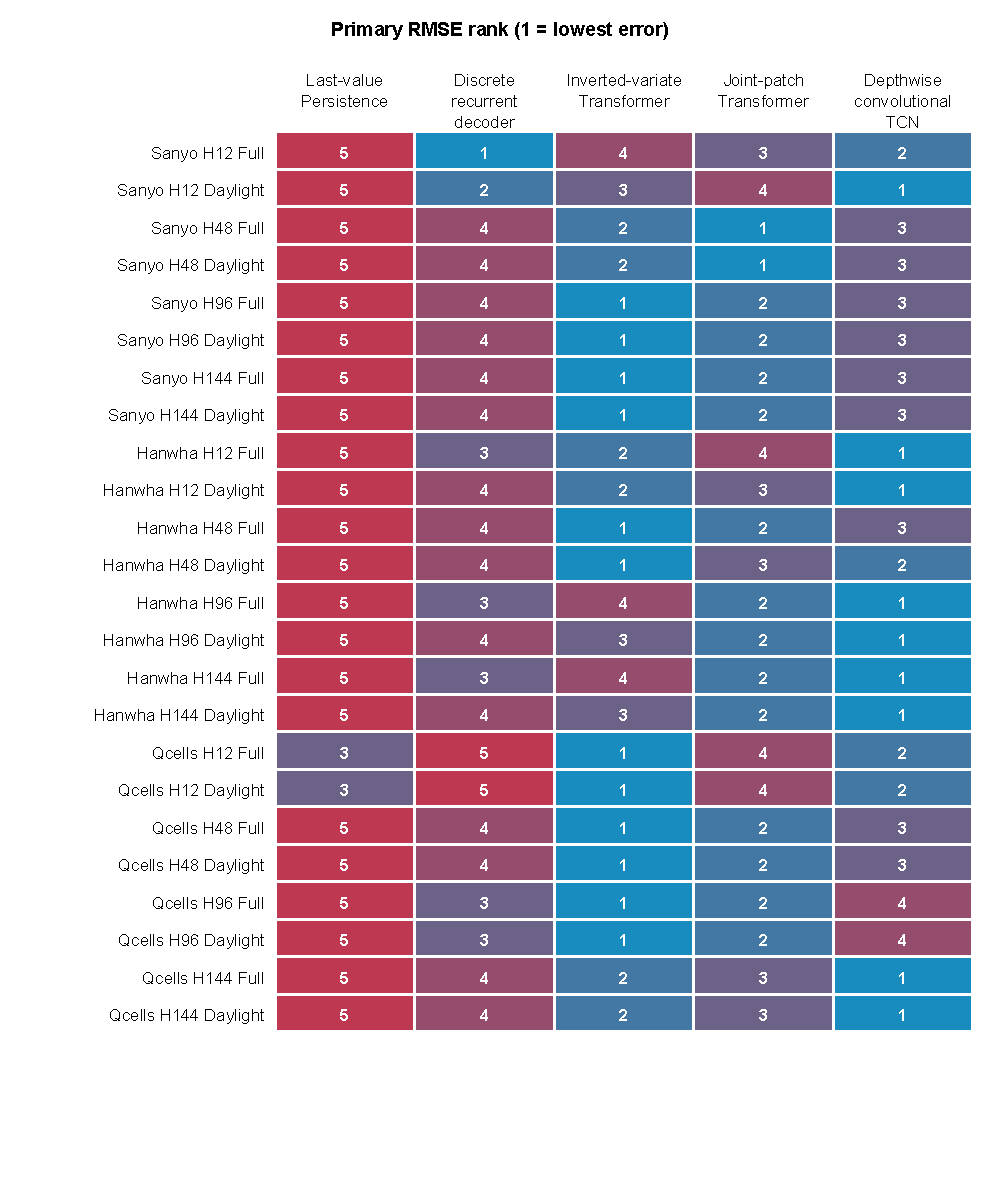
\includegraphics[width=0.86\textwidth]{figures/figS1_rank_heatmap.pdf}
\caption{RMSE ranks for all 24 primary array--horizon--scope combinations. Rank one denotes the smallest error. Short column names correspond to Last-value Persistence, Discrete recurrent decoder, Inverted-variate Transformer, Joint-patch Transformer, and Depthwise convolutional TCN.}
\label{figs:rank}
\par\small\textit{Alt text: Heat map of RMSE ranks across 24 array, horizon, and scope combinations. Columns denote Last-value Persistence, Discrete recurrent, Inverted-variate, Joint-patch, and Depthwise TCN; rankings change across conditions.}\par
\end{figure}

\section{Independent evidence verification}
An independent NumPy/Pandas verifier reads the saved H144 predictions, labels, timestamps, and validity arrays without importing the production metric or mask functions. It re-derives primary and Daily-matched masks, Persistence forecasts, RMSE, MAE, Train-range nRMSE, ranks, and sample counts. The frozen Alice audit records all 4,414 comparisons passing the registered numerical tolerances; the maximum absolute discrepancy was $8.51\times10^{-12}$ and the maximum relative discrepancy was $3.23\times10^{-11}$. The verifier confirmed primary wins of 12, 9, 2, and 1 for the Inverted-variate, Depthwise, Joint-patch, and Discrete implementations, respectively, with zero for Last-value Persistence. It also confirmed that Daily Persistence was lower than the post hoc best-of-four neural envelope in 22 comparisons; the two envelope wins were Hanwha H12 full-timeline and daylight.


\begin{figure}[p]\centering
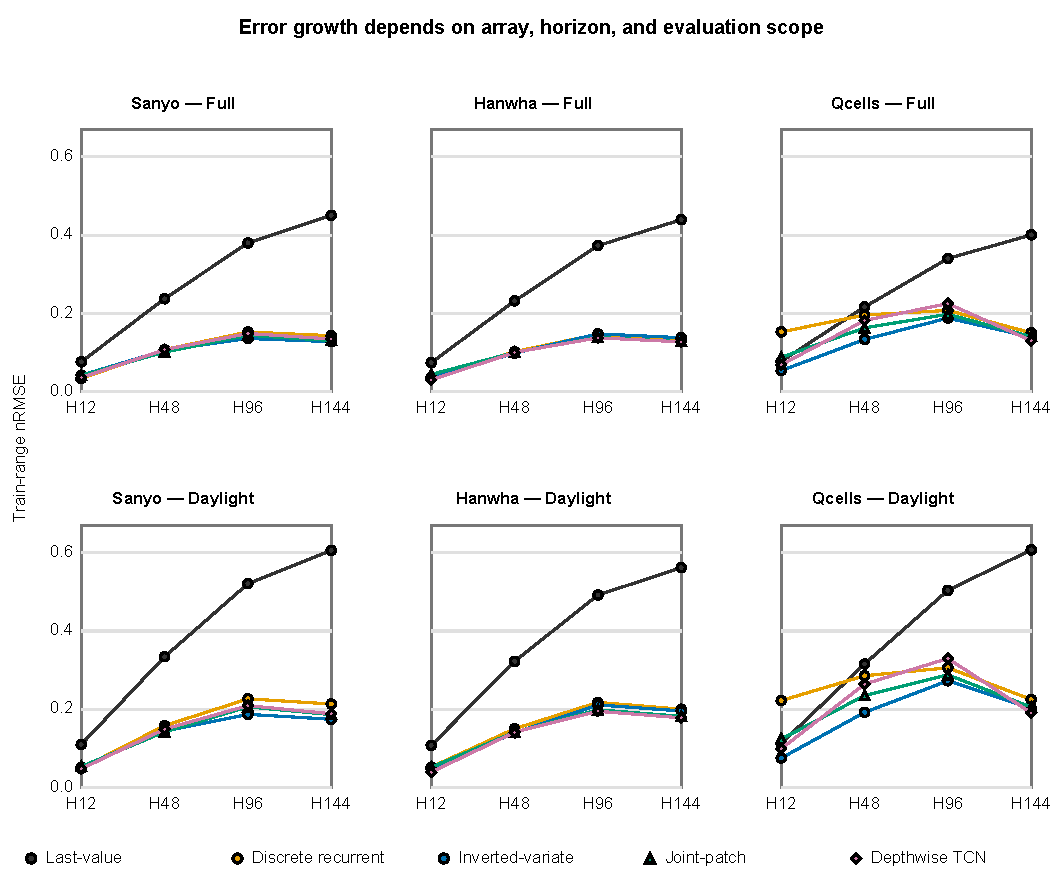
\includegraphics[width=0.97\textwidth]{figures/fig3_horizon_technology.pdf}
\caption{Alice primary Train-range nRMSE for every horizon, array, and scope.}
\label{figs:horizons}
\par\small\textit{Alt text: Six panels separate full/daylight scopes and three co-located arrays, showing all four compact models and Last-value across H12, H48, H96, and H144.}\par
\end{figure}
\begin{figure}[p]\centering
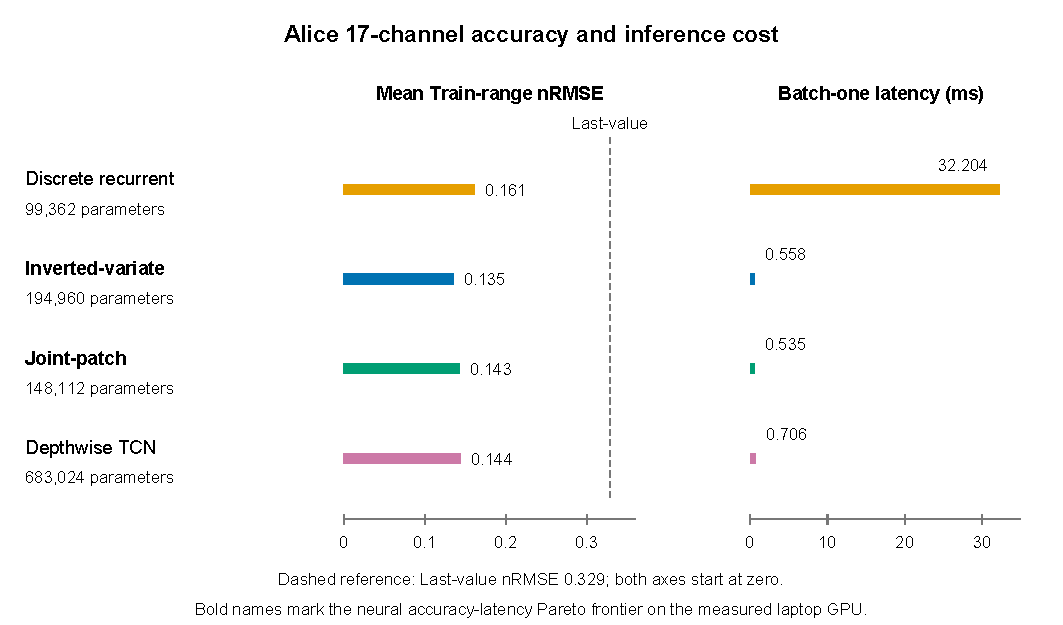
\includegraphics[width=0.85\textwidth]{figures/fig4_accuracy_efficiency.pdf}
\caption{Alice 17-channel accuracy and measured inference latency on the documented RTX 3060 Laptop GPU. Timing excludes data ingestion and preprocessing.}
\label{figs:efficiency}
\par\small\textit{Alt text: Aligned rows show parameters, average normalized error and latency for four implementations on zero-based axes. A dashed line marks Last-value error. Joint-patch is fastest and Inverted-variate has the lowest average normalized error.}\par
\end{figure}
\section{Alice inference measurement details}
Parameter counts include all learned tensors. Batch-one latency and batch-256 throughput were measured in evaluation and inference modes on an NVIDIA GeForce RTX 3060 Laptop GPU with float32 inputs of shape $[B,72,17]$. Warm-up preceded synchronized repetitions. Timing excludes model loading, disk input/output, data loading, and host-to-device transfer. Peak allocation is reported in MiB. These hardware-specific measurements support only within-environment comparisons.

\section{Unmatched-sample diagnostic}
Deleting unavailable lag points from Daily Persistence alone changes its target support and can reverse a headline comparison even when each metric is calculated correctly. The matched-support analysis applies one point mask to Daily Persistence, Last-value Persistence, every neural seed, and the labels. Unmatched-support values are therefore treated only as a methodological diagnostic and never as model-performance evidence.

\end{document}
